\documentclass[letterpaper, 10 pt, conference]{ieeeconf}  % Comment this line out if you need a4paper

\IEEEoverridecommandlockouts                             
\overrideIEEEmargins

\usepackage[utf8]{inputenc}
\usepackage[T1]{fontenc}
\usepackage{graphicx}
\usepackage{float}
\usepackage{xcolor}

\usepackage{amsmath}
\usepackage{amsfonts}
\usepackage{amssymb}

\newcommand{\ph}[1]{{\textbf{#1}:}} % paragraph header
\newcommand{\todo}[1]{{\color{red} #1 }} % Tasks to do

\newcommand{\argmax}{\mathop{\mathrm{argmax}}}
\newcommand{\argmin}{\mathop{\mathrm{argmin}}}


\title{\LARGE \bf
Perception-aware and Risk-cognizant Planning Under Uncertainty for Autonomy in Extreme Environments
}


\begin{document}
\maketitle
\thispagestyle{empty}
\pagestyle{empty}


\begin{abstract}
In this work, we propose a framework for planning under uncertainty that bridges the gap between high-fidelity continuous traversability analysis and discrete behavior planning.
\end{abstract}


%%%%%%%%%%%%%%%%%%%%%%%%%%%%%%%%%%%%%%%%%%%%%%%%%%%%%%%%%%%%%%%%%%%%%%%%%%%%%%%%
% \ph{Paragraph header} Please start every single paragraph with a paragraph header, summarizing the intention of that paragraph. This is mainly for iterations during the paper preparation. We will remove most of them for the final report.

\section{Questions}
\begin{itemize}
    \item what is the best map representation (continuous/grid)
    \item what is the best representation for "occupancy" in the map - is it (free/unknown/occupied) vs risk (0,1)?  also include artifact presence or probability of artifact presence.
    \item robot pose 3d? yaw?  quaternion?
    \item information gain - how to interpret in IRM level?  total number of breadcrumbs?
    \item 
\end{itemize}

\subsection{information gain brainstorming}
\begin{itemize}
    \item \# of breadcrumbs
    \item 2d number of cells
    \item 3d number voxels
    \item mesh \# facets, surfaces (observed)
    \item volume in 3d..
    \item area of raytrace, area of coverage...
\end{itemize}
eventually we want to abstract this into IRM level.  need a happy marriage between high res info with irm abstraction.\\

\subsection{How to decouple problem}
\begin{itemize}
    \item \# new breadcrumbs (current implementation)
    \item 
\end{itemize}

%%%%%%%%%%%%%%%%%%%%%%%%%%%%%%%%%%%%%%%%%%%%%%%%%%%%%%%%%%%%%%%%%%%%%%%%%%%%%%%%
\section{Introduction}
\ph{Real world example} Consider a robot tasked to map a GPS-denied area in moving under time constraints. 


%%%%%%%%%%%%%%%%%%%%%%%%%%%%%%%%%%%%%%%%%%%%%%%%%%%%%%%%%%%%%%%%%%%%%%%%%%%%%%%%
\section{Related Work}


%%%%%%%%%%%%%%%%%%%%%%%%%%%%%%%%%%%%%%%%%%%%%%%%%%%%%%%%%%%%%%%%%%%%%%%%%%%%%%%%
\section{Background}

%% (excerpted from Sung's thesis)

In this section we briefly introduce generic POMDP formulation.
For a detailed information, see e.g.,~\cite{Bertsekas05,TBF05,RN10}

Let $\mathbb{S}$, $\mathbb{A}$, and $\mathbb{Z}$ denote the state, action, and observation spaces, respectively.
We denote the motion model $T(s, a, s') = P(s'\,|\,s, a)$, which defines the probability of being at state $s'$ after taking an action $a$ in state $s$.
The observation model $Z(s, a, z) = P(z\,|\,s, a)$ is the probability of receiving observation $z$ after taking action $a$ in state $s$. 

A belief $b(s)$ is a posterior distribution over all possible states given the past actions and observations, i.e., $b_{k}(s) = P(s \,|\, a_{0:k-1}, o_{1:k})$ where the subscript $k$ denotes the time step.
Note that a POMDP problem can be formulated as a \textit{Belief MDP} by taking $b(s)$ as an MDP state, also referred to as a \textit{belief state} $b \in \mathbb{B}$, where $\mathbb{B}$ is referred to as \textit{belief space}.

Given $a_{k-1}$, $z_k$, and $b_{k-1}(s)$,
the updated belief $b_k(s)$ can be computed by Bayesian filtering, which can be divided into two sub-steps as follows.
\begin{align}
  b_{k-1}(s; a_{k-1}) &= \sum_{s' \in \mathbb{S}} T(s, a_{k-1}, s') b_{k-1}(s),
  \label{eq:prediction}
  \\
  b_k(s; a_{k-1}, z_k) &= \eta Z(s, a_{k-1}, z_k) b_{k-1}(s; a_{k-1}),
  \label{eq:correction}
\end{align}
where $\eta$ is a normalizing constant.
For notational convenience, let us denote $b_{k-1}(s; a) = b_{k-1}^a$ and $b_k(s; a, z) = b_k = b_{k-1}^{a z}$ hereafter.

A policy $\pi : \mathbb{B} \rightarrow \mathbb{A}$ maps each belief state $b$ to a desirable action $a$.
The expected cost of an action for the true state can be represented as a cost function in a belief space, $c(b, a) \in \mathbb{R}^+$.
Given a policy $\pi$ and a belief $b \in \mathbb{B}$, we can compute the value function,
\begin{align}
  J(b; \pi) %= \mathbb{E} \left[ \sum_{k=0}^\infty \gamma^k c(b_k, a_k); \pi \right]
  = \mathbb{E} \left[ \sum_{k=0}^\infty \gamma^k c(b_k, \pi(b_k)) \right]\!,
  \label{eq:trueV}
\end{align}
where $b_0$ is the initial belief state and 	$\gamma \in (0, 1]$ is a discount factor that reduces the effect of later costs.


We can rewrite Eq.~\ref{eq:trueV} in a recursive form, which is called the Bellman equation.
\begin{align}
J(b; \pi) = c(b^i, \pi(b)) % \nonumber \\
   + \gamma \sum_{b' \in \mathbb{B}} \tau(b, \pi(b), b') J(b'; \pi),
  \label{eq:bellman}
\end{align}
where $\tau(b, \pi(b), b') = \sum_{z \in \mathbb{Z}} P(b'|b,\pi(b),z) P(z|b,\pi(b))$ is the transition probability from $b$ to $b'$ under $\pi$,
which can be derived from Eq.~\ref{eq:prediction} and~\ref{eq:correction}.
For further details, see~\cite{Ross08}.

It is often convenient to define the so-called Q-value function for an intermediate belief-action pair, $(b, a)$ or simply $b^a$, as follows.
\begin{align}
  Q(b^a; \pi) =\; & c(b, a) + \gamma \sum_{b' \in \mathbb{B}} \tau(b, a, b') J(b'; \pi).
  \label{eq:qfunction}
\end{align}
Then Eq.~\ref{eq:bellman} can be written as follows.
\begin{align}
J(b; \pi) =\; & \min_{a \in \mathbb{A}} Q(b, a; \pi)
\label{eq:minq}
\end{align}

We now restate our POMDP problem as an optimization problem.
\begin{align}
  \pi^*(b) & = \argmin_{\Pi_{0:\infty}} \mathbb{E} \left[ \sum_{k=0}^\infty \gamma^k c(b_k, \pi_k(b_k)) \right]
  \nonumber \\ 
  &  = \argmin_{\Pi_{0:\infty}} J(b_k; \pi_k).
  \label{eq:optonline}
\end{align}


%%%%%%%%%%%%%%%%%%%%%%%%%%%%%%%%%%%%%%%%%%%%%%%%%%%%%%%%%%%%%%%%%%%%%%%%%%%%%%%%
\section{Problem Formulation}

In this section, we formulate our autonomous exploration problem in unknown environments.
The high-level objective of our problem is to \textit{cover} the unexplored space as much as possible for the given time.

It can be formulated as an optimization problem as follows.
\begin{align}
  \pi^*(b) & = \argmax_{\Pi_{0:T}} \mathbb{E} \left[ \sum_{k=0}^T I(b_k, \pi_k(b_k)) \right],
\end{align}
where $I(b, \pi(b))$ denote \textit{information gain} after taking an action at $b$ under $\pi$,
and $T$ is the allowed time for autonomous exploration.



%%%%%%%%%%%%%%%%%%%%%%%%%%%%%%%%%%%%%%%%%%%%%%%%%%%%%%%%%%%%%%%%%%%%%%%%%%%%%%%%
\section{Problem Formulation}
Let $s$, $\pi_f$, and $M$ denote the robot's state, a move-to-frontier action, and map, respectively. We formulate the coverage objective function as the ratio of newly sensed map information ($B$) to the temporal cost of sensing this information ($c_t$), both of which are functions of the transition function $T(s,\pi_f,M)$.

\begin{align}
    J^{cov}(s,\pi_f,M) &= \frac{B[T(s,\pi_f,M)]}{c_t[T(s,\pi_f,M)]} \\ \nonumber \\ 
    T &\colon s \times \pi_f \times M\to \tau \nonumber \\
    B &\colon \tau\to \Delta n_{bc} \nonumber \\
    c_t &\colon s \times \pi_f \times M\to \Delta t \nonumber 
\end{align}

\noindent where, for a given the move-to-frontier action $\pi_f$, $\tau$ is the robot trajectory, $\Delta t$ is duration of traversal, and $\Delta n_{bc}$ is the number of new breadcrumbs added to the IRM. We select an action $\pi_f$ which maximizes our coverage objective function:
\begin{align}
    % f^* &= \arg\max_{f\in F}_{~~\tau \in \Gamma} J^{cov}(s,f,M) \\
    \pi_f^* &= \arg\max_{\substack{\pi_f\in \Pi_f \\ \tau \in T}} J^{cov}(s,f,M) \\
    s.t.~~&~\textrm{risk}(s,\pi_f,M)< \psi(t)
\end{align}

\noindent The risk (or probability of traversal) associated with the optimal action is required to be smaller than a time adaptive threshold. As the duration of the mission progresses, the risk threshold $\psi(t)$ increases to allow for riskier actions.

% Let $x_k$, $u_k$, and $z_k$ denote the robot state, action, and observation at the $k$-th time step.
% \begin{align}
%     \pi^* &= \arg\min_{\pi\in \Pi} J(?, ?, \pi) \\
%     s.t.~~&~constraint 1 \\
%     ~ &~constraint 2
% \end{align}

\subsection{Defining risk}
It is easier to define risk as the probability of success, rather than the probability of failure, since for the mission to succeed, we require the intersection of multiple successful events.  Let $r(s,\pi_f,M,t)$ be the probability of success associated at each (timestep?  transition?), which we define as the probability that the robot does not fail or crash for that interval.  We define the total \emph{mission risk} $R$ as the probability that the robot does not fail over the entire mission.  For a given mission duration $D$, the mission risk is given by:
\begin{equation}
    R= \prod_{t=0}^D risk(s,\pi_f,M,t)
\end{equation}
In general, risk may be a function of the state $s$, actions $\pi_f$, and map $M$.  We can make the simplifying assumption that is is a function each grid cell within the map $m_i$.  (is $m_i$ the occupancy value or the grid itself?  or is $i$ indication the grid?)  Let $m_i(t)$ be the grid cell that the robot occupies at time $t$.  Then we have $risk(m_i(t)) = \prod_{k} r_k(m_i(t))$ where we have $k$ risk factors.  Each risk factor may be due to a different source of potential failure, e.g. rough terrain, proximity to obstacles, slope, slippery/muddy terrain, etc.  For computational tractability we can compute the log mission risk: 
\begin{equation}
    \log R=\bigg[\sum_{t=0}^D\sum_{k} \log(r_k(m_i(t)))\bigg] > \Phi
\end{equation}
which we want to constrain to be above some total acceptable mission risk threshold $\Phi$.
\section{Problem Solution}

\subsection{Local Selection}

\begin{itemize}
  \item Objective 1: Connect local to global coverage
  \begin{itemize}
  \item In-depth path planning to selected frontier
  \item Expectation Model or leaf-node heuristic function
  \end{itemize}
  \item Objective 2: More robust traversability (no oscillations!)
  \begin{itemize}
  \item Way-point assignments 
  \end{itemize}
\end{itemize}


%%%%%%%%%%%%%%%%%%%%%%%%%%%%%%%%%%%%%%%%%%%%%%%%%%%%%%%%%%%%%%%%%%%%%%%%%%%%%%%%
\section{Environment representation}
\subsection{Occupany Grid Mapping}
Given a set of observations taken at known robot poses, the posterior over maps is given by:
\begin{align}
    p(m | z_{1:t},x_{1:t})
\end{align}
\noindent where $m$ is the map, $z_{1:t}$ is the set of all measurements up to time $t$, and $x_{1:t}$ is path of robot. 
Occupancy grid map is composed of grid cells:
\begin{align}
    m = \{\textbf{m}_i\}
\end{align}
\noindent where $\textbf{m}_i$ is associated with a binary occupancy value indicating whether cell is occupied or free. Calculating the posterior for every single map is intractable, therefore, problem can be formulated as the posterior over a single grid cell: 
\begin{align}
    p(\textbf{m}_i | z_{1:t},x_{1:t})
\end{align}
Here, we are estimating a fixed, binary state that does not change over time. When the state is static, posterior is only function of measurements:
\begin{align}
    p(\textbf{m}_i | z_{1:t},x_{1:t}) = p(\textbf{m}_i | z_{1:t})
    \label{static}
\end{align}
This problem can be addressed by the Binary Bayes filter. The \emph{odds} of a state $\textbf{m}_i$ is defined as the ratio of the probability that the cell is free to that of the cell being occupied:
\begin{align}
    \frac{p(\textbf{m}_i | z_{1:t},x_{1:t})}{1-p(\textbf{m}_i | z_{1:t},x_{1:t})}
    \label{odd}
\end{align}
The \emph{log odds} is the logarithm of this ratio:

\begin{align}
    l_{t,i} = \log\frac{p(\textbf{m}_i | z_{1:t},x_{1:t})}{1-p(\textbf{m}_i | z_{1:t},x_{1:t})}
    \label{log_odd}
\end{align}
An inverse measurement model, $p(\textbf{m}_i | z_{1:t},x_{1:t})$, which specifies the distribution over the binary state variable $\textbf{m}_i$ as a function of the measurement $z_{1:t}$, is used since the measurements are much more complex than the binary state. 
\noindent By rearranging Eq. \ref{log_odd}, the posterior over the grid cell is exposed:
\begin{align}
    p(\textbf{m}_i | z_{1:t},x_{1:t}) = 1-\frac{1}{1+\exp(l(\textbf{m}_i))}
\end{align}
\noindent Eq. \ref{log_odd} can be expanded in accordance with Bayes filter:
\begin{align}
    l_{t,i} &= \log\frac{p(\textbf{m}_i | z_{t},x_{t})}{1-p(\textbf{m}_i | z_{t},x_{t})} - \log\frac{p(\textbf{m}_i | z_{1:t-1}, x_{1:t-1})}{1-p(\textbf{m}_i | z_{1:t-1}, x_{1:t-1})} \nonumber \\
    &\quad - \log\frac{p(\textbf{m}_i)}{1-p(\textbf{m}_i)} \nonumber \\
    &= l_{t-1,i} + \log\frac{p(\textbf{m}_i | z_{t},x_{t})}{1-p(\textbf{m}_i | z_{t},x_{t})} + l_{0,i}
\end{align}
\noindent where $l_{t-1,i}$ is the previous log-odds value, $l_{0,i}$ is the log-odds representation of the occupancy prior $p(\textbf{m}_i)$, and $p(\textbf{m}_i | z_{t},x_{t})$ is the inverse sensor model.

However, this formulation does not reflect dependencies among neighboring cells. 

\subsection{Information Gain}
Entropy is a measure for the the uncertainty of a posterior. The entropy $H_p(x)$ of a probability distribution $p$ is the expected information $E[-\log p]$. The entropy of the occupancy grid map posterior is
\begin{align}
    H_p(\textbf{m}_i) = -p(\textbf{m}_i) \log p(\textbf{m}_i) - (1-p(\textbf{m}_i)) \log(1-p(\textbf{m}_i))
\end{align}
\noindent and the expected entropy after measuring is $E[H_{p}(\textbf{m}_i)]$. Then the expected information gain when sensing a grid cell $\textbf{m}_i$ is: 
\begin{align}
    I_i = H_p(\textbf{m}_i) - E[H_{p}(\textbf{m}_i)]
\end{align}



%%%%%%%%%%%%%%%%%%%%%%%%%%%%%%%%%%%%%%%%%%%%%%%%%%%%%%%%%%%%%%%%%%%%%%%%%%%%%%%%
\section{Risk quantification}
In this section, we discuss how we associate risk and cost values to a given trajectory in the environment.

%%%%%%%%%%%%%%%%%%%%%%%%%%%%%%%%%%%%%%%%%%%%%%%%%%%%%%%%%%%%%%%%%%%%%%%%%%%%%%%%
\section{Frontier-based Coverage Planning}

\subsection{IRM}



\subsection{Frontier Detection}

\subsubsection{Frontier map}
\todo{David} How we represent 3D lidar data in 2D frontier map
\begin{itemize}
    \item We want to capture traversability information here
    \item We can include a full discussion about traversability analysis, computing risk metrics for traversal, and capturing known vs. unknown regions
    \item We can fold in the current writeup on traversability here, then add additional risk/traversability metrics
\end{itemize}
\subsubsection{Frontier detection}
\todo{Sung} Frontier detection algorithm


\subsection{Frontier Maintenance}
\todo{Sung} Frontier node maintenance details

%%%%%%%%%%%%%%%%%%%%%%%%%%%%%%%%%%%%%%%%%%%%%%%%%%%%%%%%%%%%%%%%%%%%%%%%%%%%%%%%
\section{Experiments}


%%%%%%%%%%%%%%%%%%%%%%%%%%%%%%%%%%%%%%%%%%%%%%%%%%%%%%%%%%%%%%%%%%%%%%%%%%%%%%%%
\section{Conclusion}




% %%%%%%%%%%%%%%%%%%%%%%%%%%%%%%%%%%%%%%%%%%%%%%%%%%%%%%%%%%%%%%%%%%%%%%%%%%%%%%%%
% \section{Instructions}
% \ph{Paragraph header} Please start every single paragraph with a paragraph header, summarizing the intention of that paragraph. This is mainly for iterations during the paper preparation. We will remove most of them for the final report.

% %%%%%%%%%%%%%%%%%%%%%%%%%%%%%%%%%%%%%%%%%%%%%%%%%%%%%%%%%%%%%%%%%%%%%%%%%%%%%%%%
% \section{Introduction}
% \ph{Real world example} Consider a robot tasked to map a GPS-denied area in moving under time constraints. 

% %%%%%%%%%%%%%%%%%%%%%%%%%%%%%%%%%%%%%%%%%%%%%%%%%%%%%%%%%%%%%%%%%%%%%%%%%%%%%%%%
% \section{Problem Formulation}
% Let $x_k$, $u_k$, and $z_k$ denote the robot state, action, and observation at the $k$-th time step.


% %%%%%%%%%%%%%%%%%%%%%%%%%%%%%%%%%%%%%%%%%%%%%%%%%%%%%%%%%%%%%%%%%%%%%%%%%%%%%%%%
% \section{Map Representation}


% %%%%%%%%%%%%%%%%%%%%%%%%%%%%%%%%%%%%%%%%%%%%%%%%%%%%%%%%%%%%%%%%%%%%%%%%%%%%%%%%
% \section{Something of Map Posterior}

% %%%%%%%%%%%%%%%%%%%%%%%%%%%%%%%%%%%%%%%%%%%%%%%%%%%%%%%%%%%%%%%%%%%%%%%%%%%%%%%%
% \section{Planning}

% %%%%%%%%%%%%%%%%%%%%%%%%%%%%%%%%%%%%%%%%%%%%%%%%%%%%%%%%%%%%%%%%%%%%%%%%%%%%%%%%
% \section{Experiments}


% %%%%%%%%%%%%%%%%%%%%%%%%%%%%%%%%%%%%%%%%%%%%%%%%%%%%%%%%%%%%%%%%%%%%%%%%%%%%%%%%
% \section{Conclusion}



\section*{APPENDIX}


\clearpage{}
\begin{figure}[H]
  \centering
  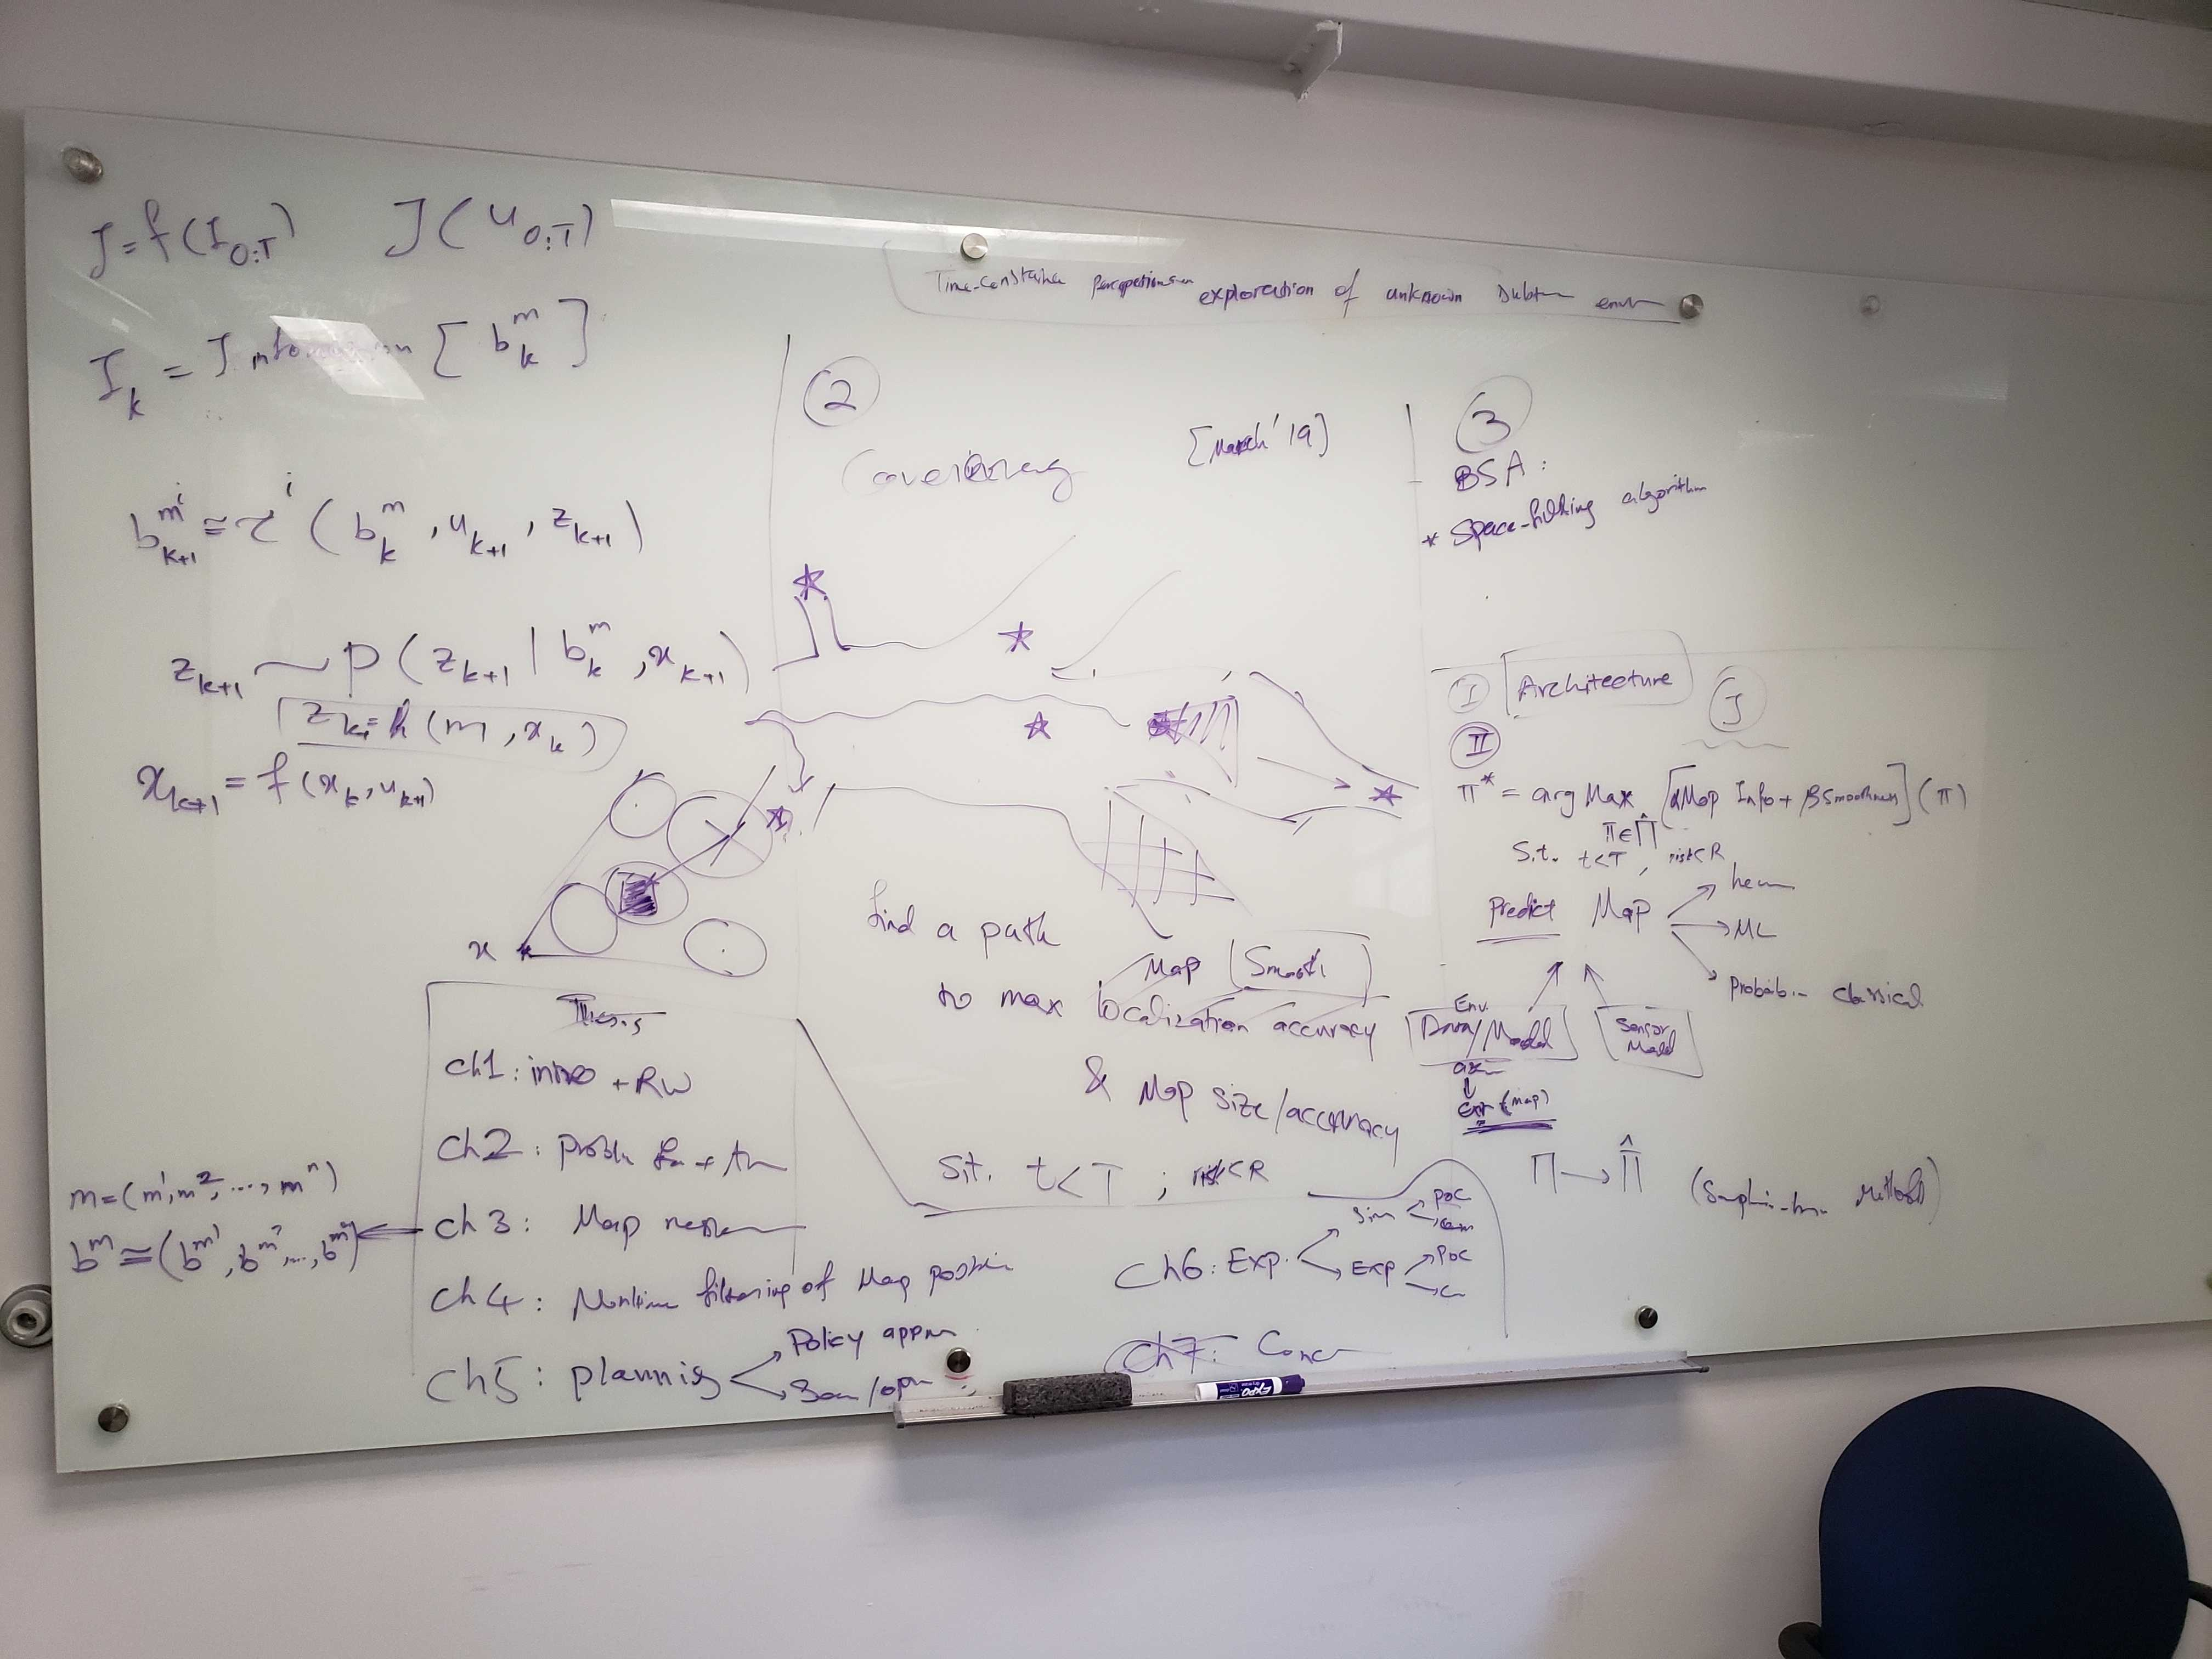
\includegraphics[width=.5\textwidth]{figures/whiteboard1.jpg}
  \label{fig:whiteboard1}
\end{figure}

\begin{figure}[H]
  \centering
  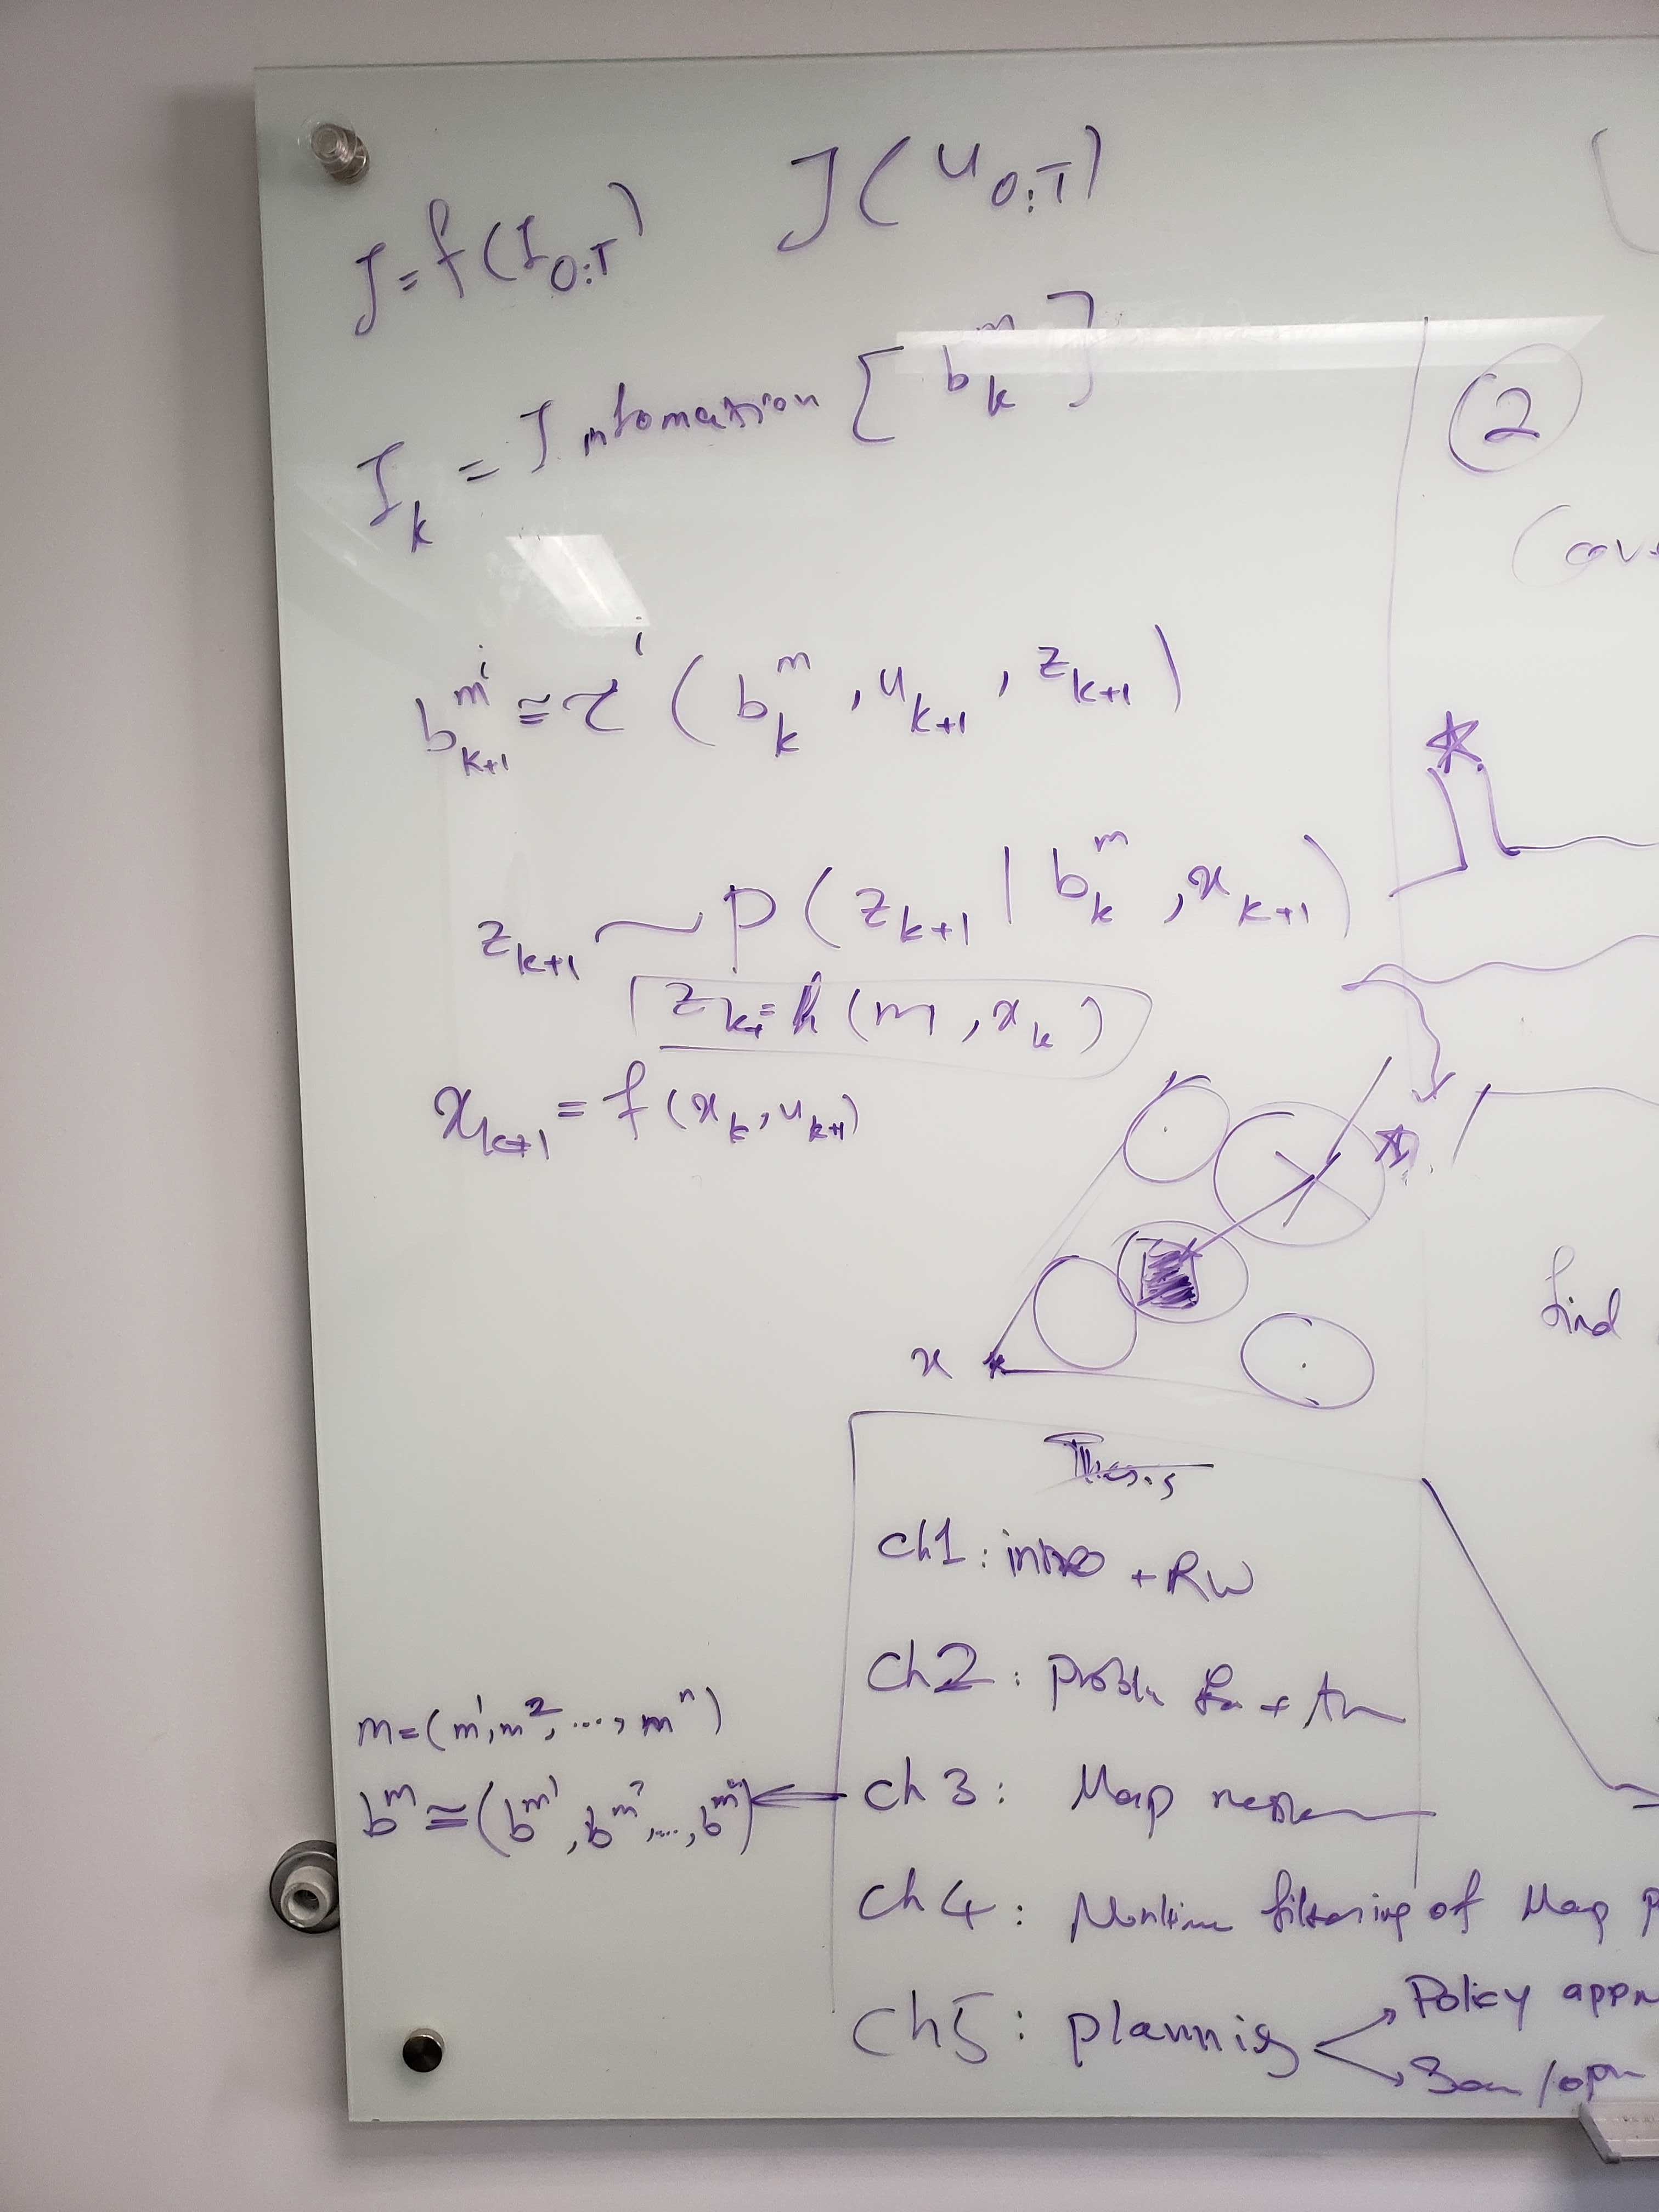
\includegraphics[width=.5\textwidth]{figures/whiteboard2.jpg}
  \label{fig:whiteboard1}
\end{figure}

\begin{figure}[H]
  \centering
  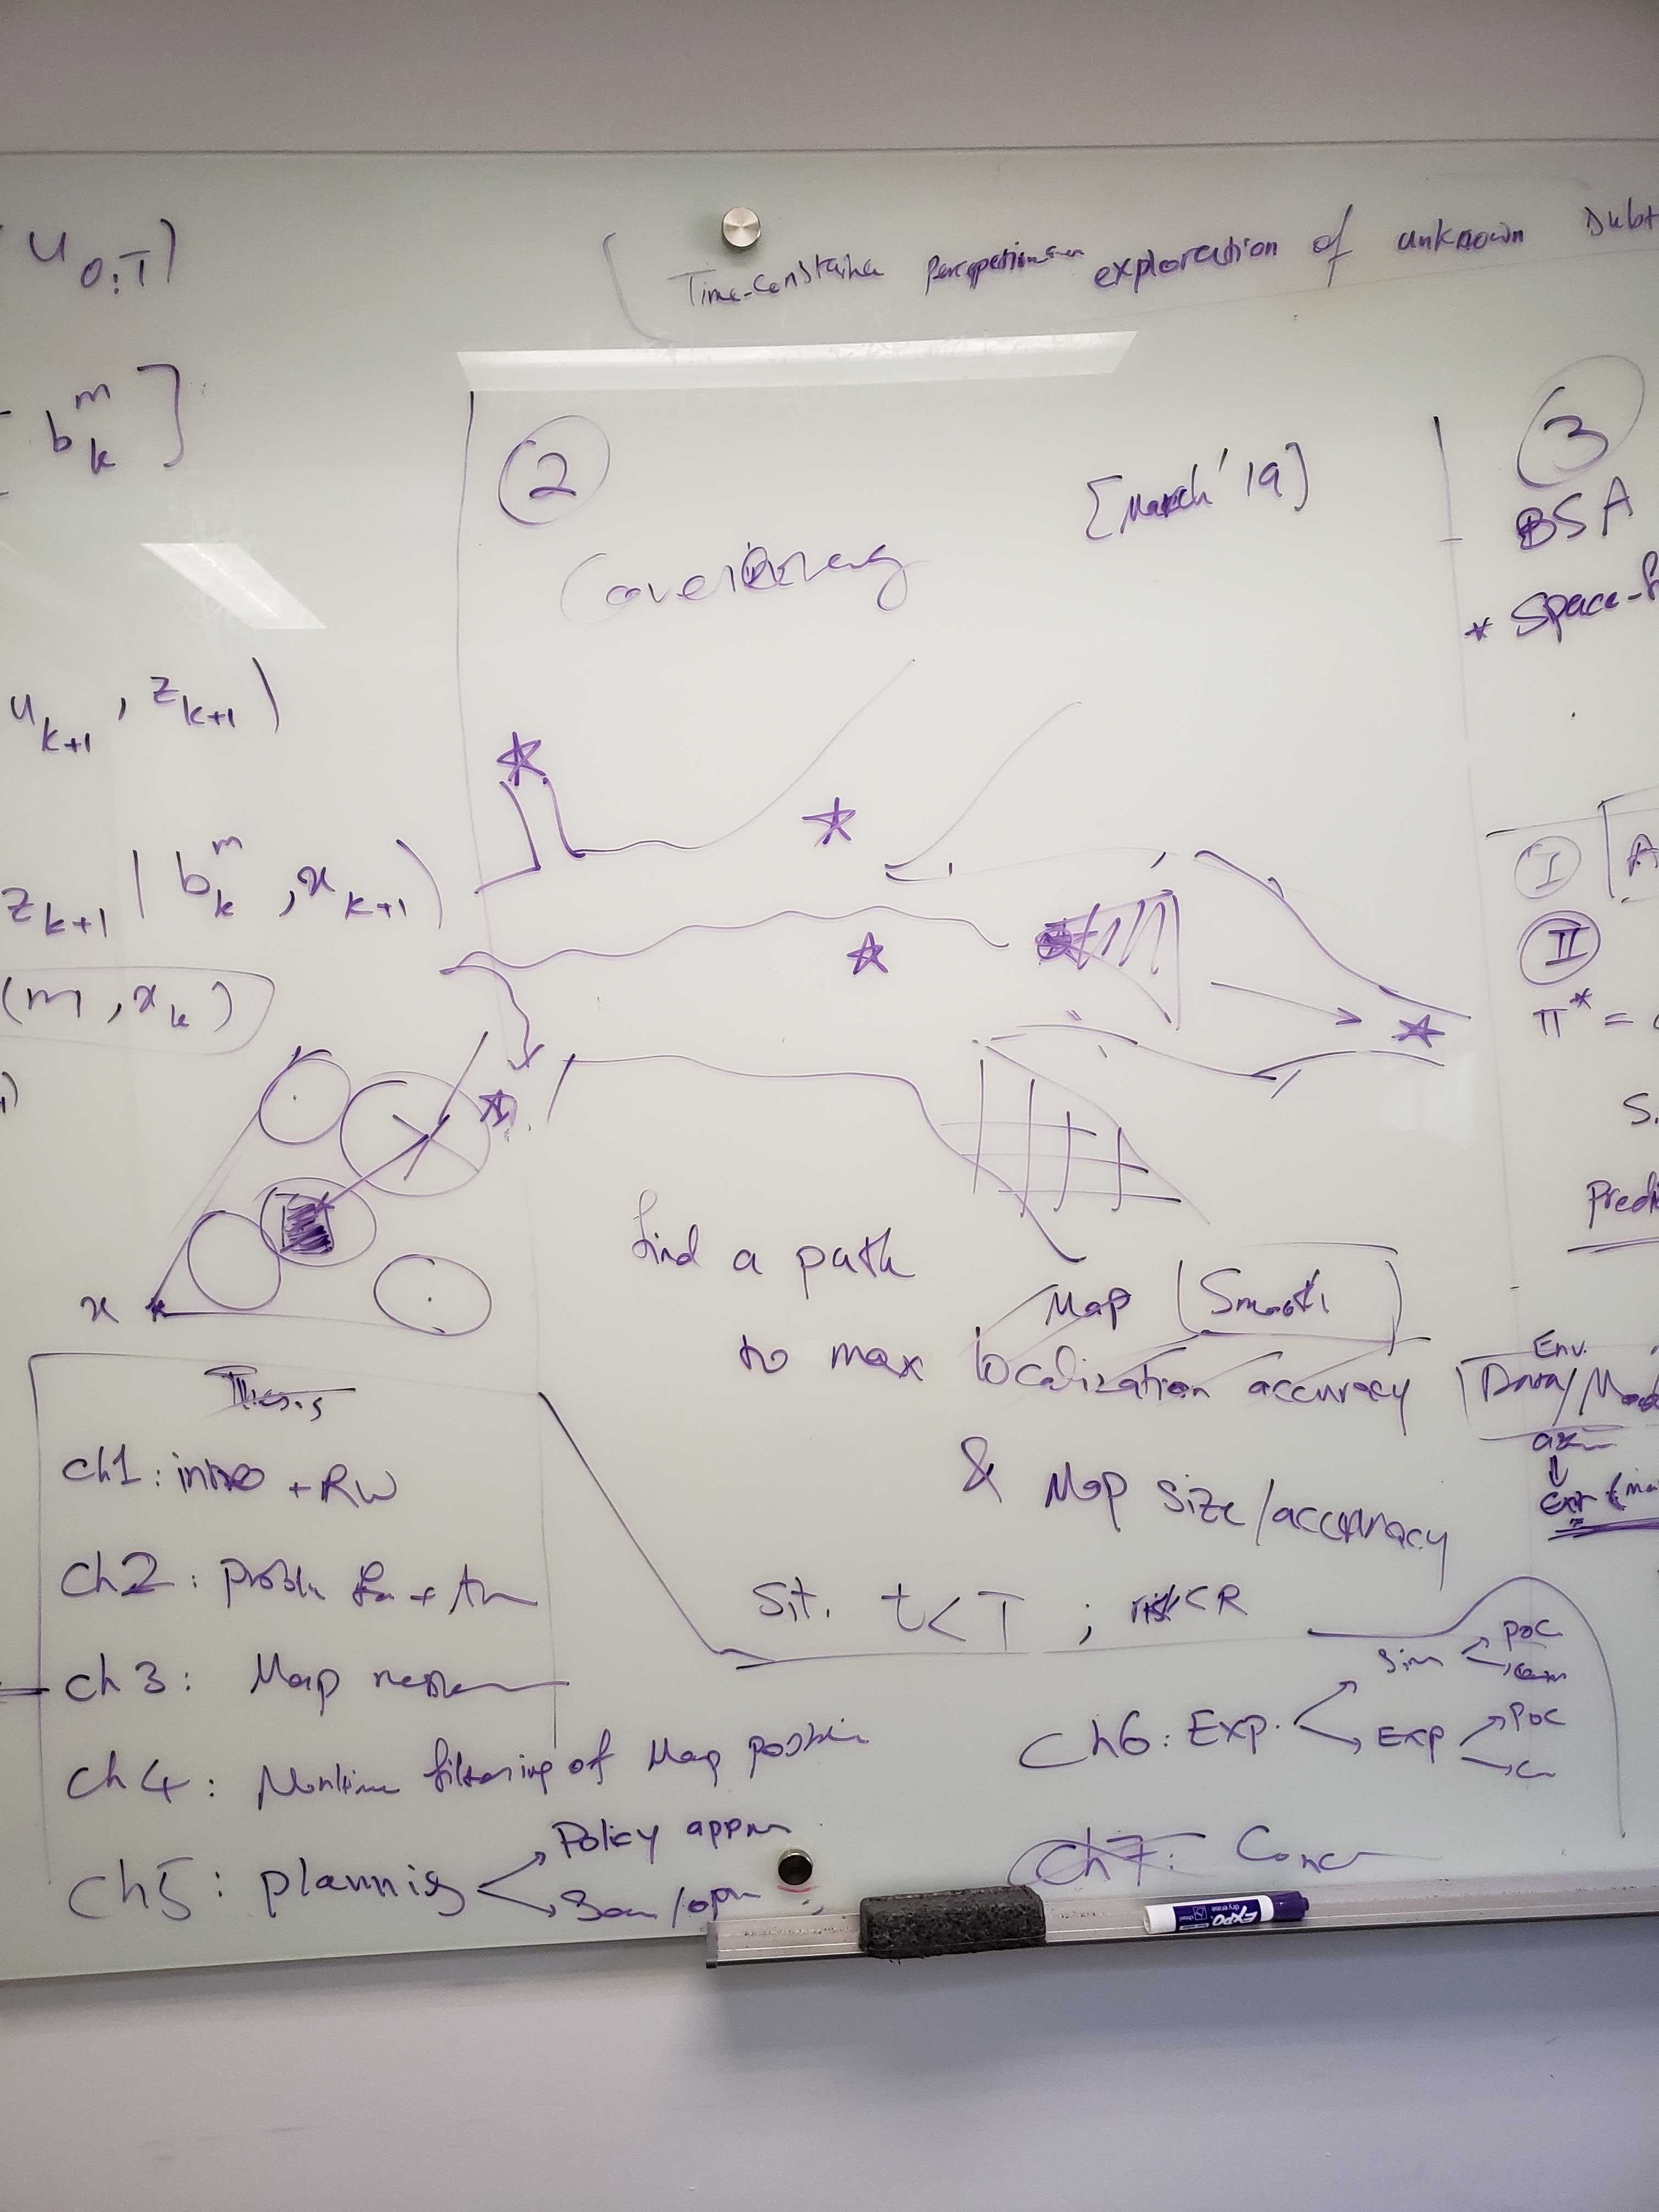
\includegraphics[width=.5\textwidth]{figures/whiteboard3.jpg}
  \label{fig:whiteboard1}
\end{figure}

\begin{figure}[H]
  \centering
  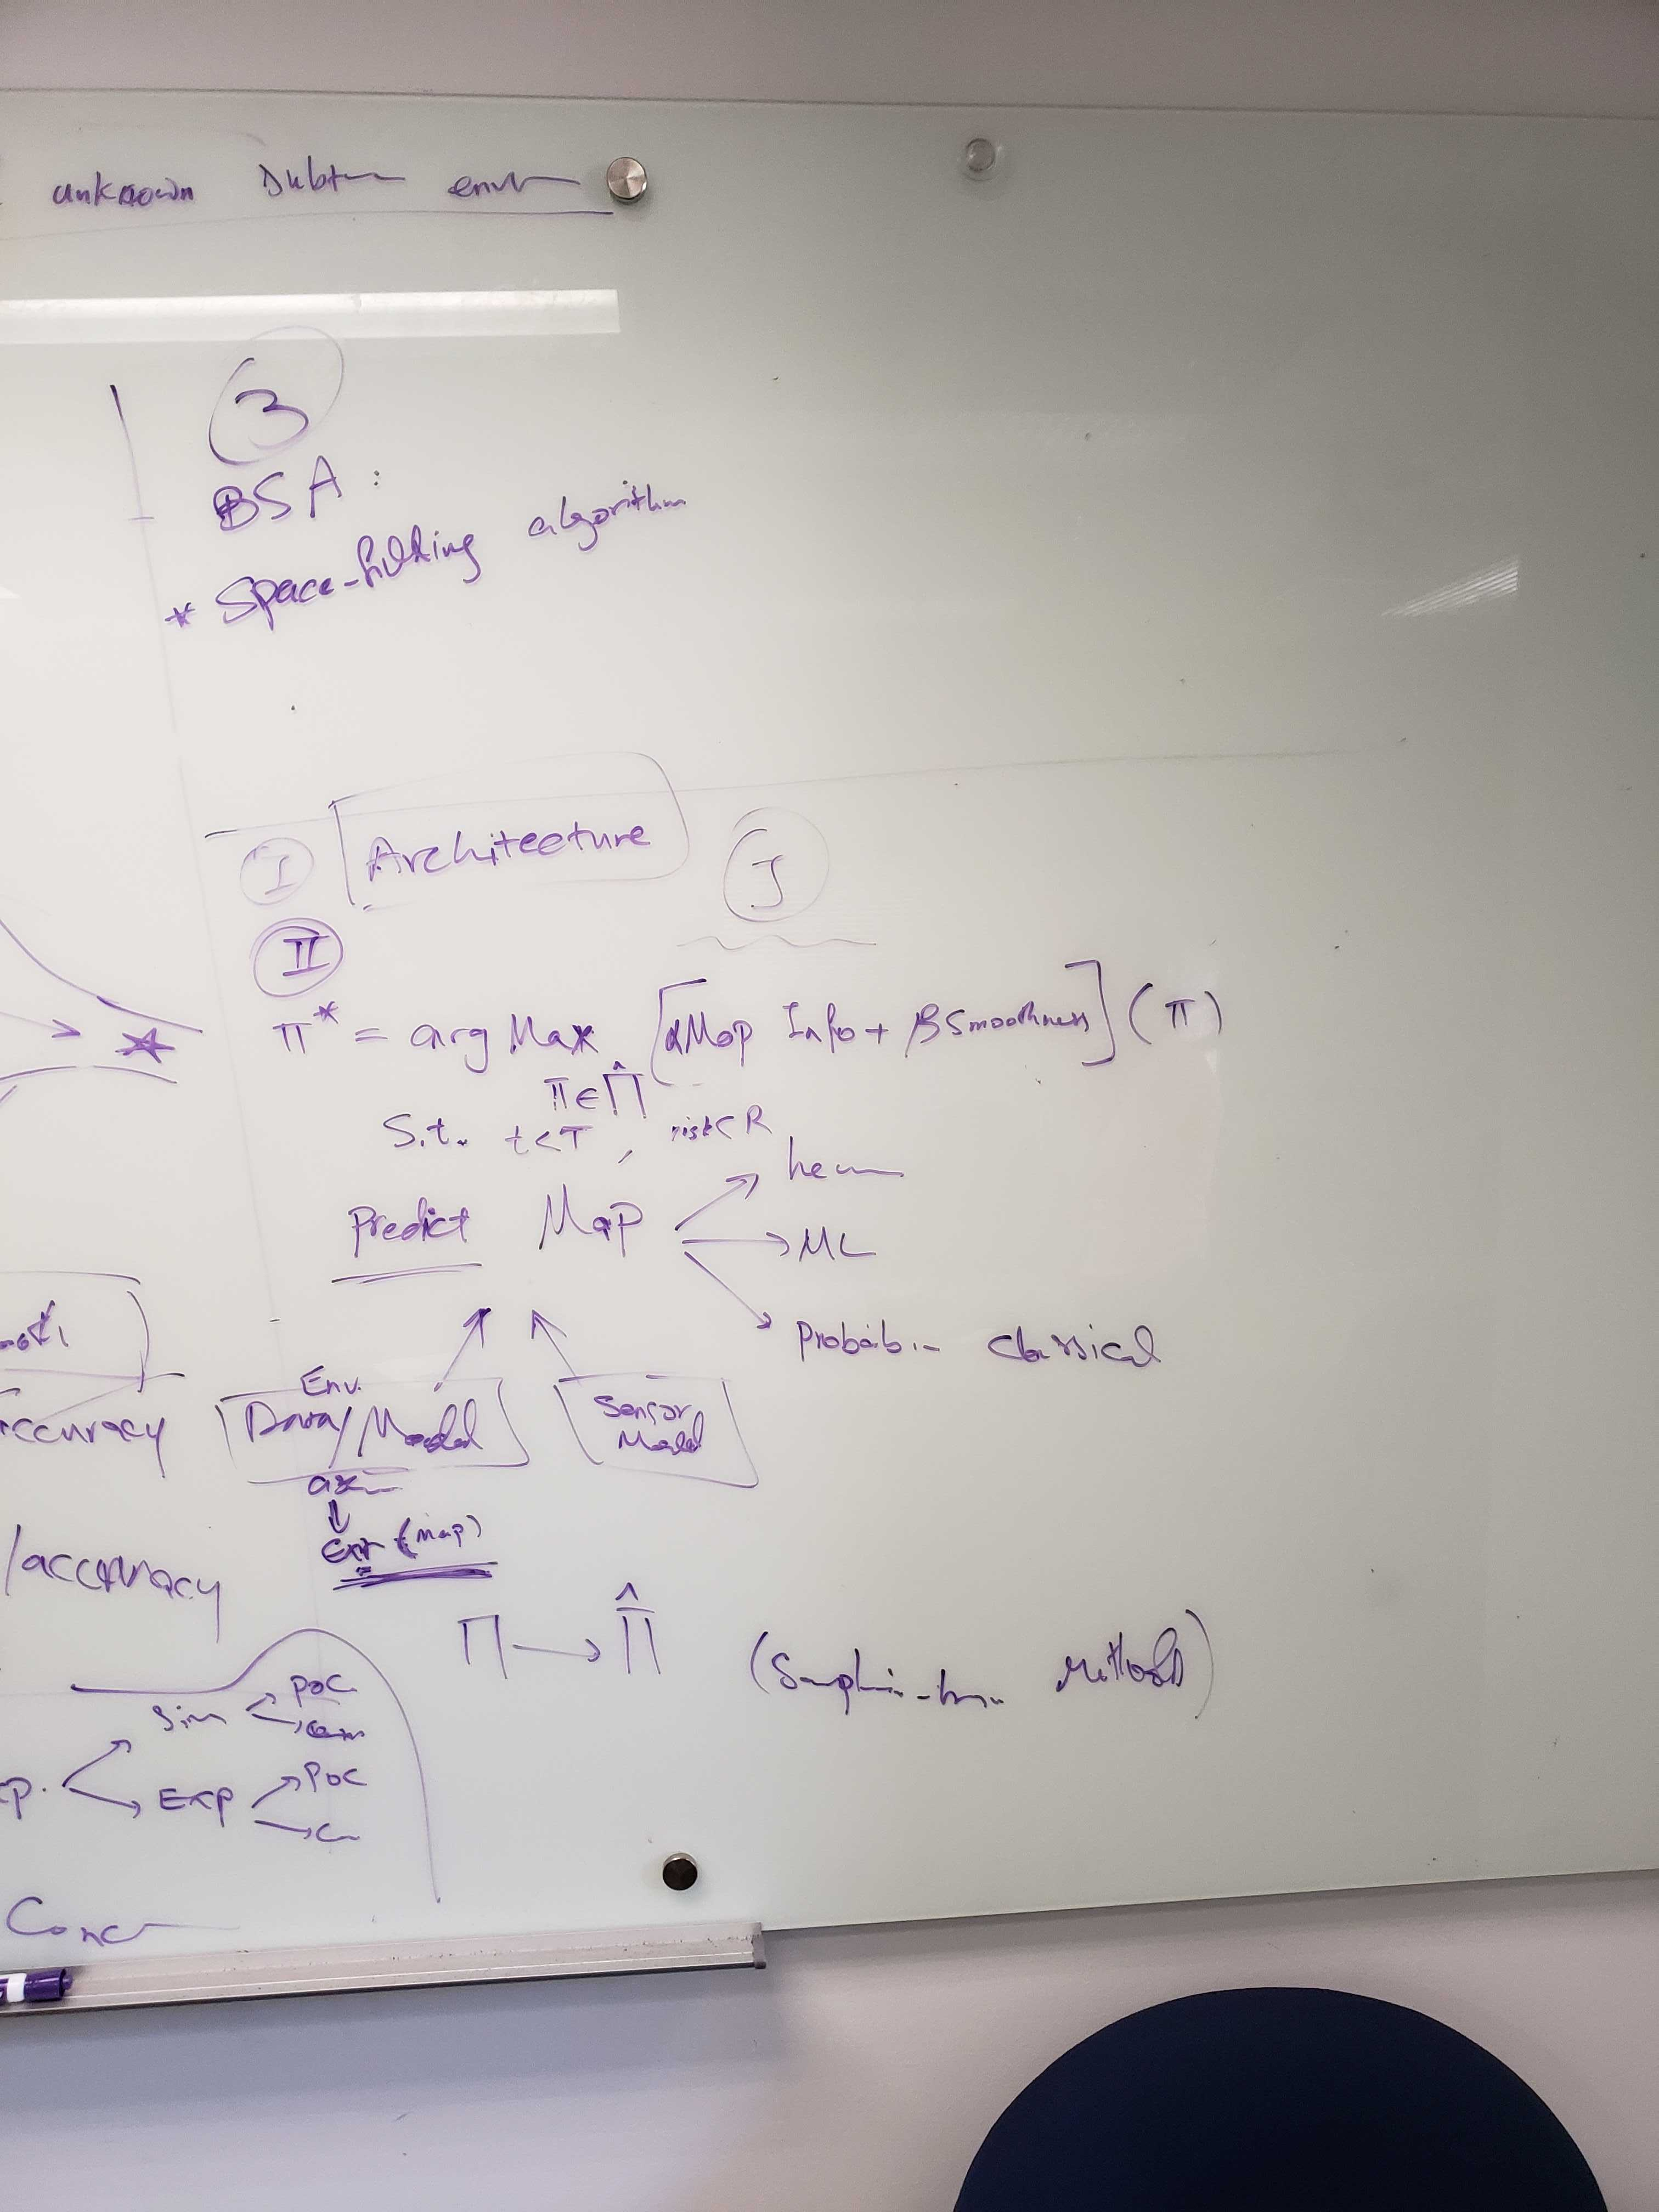
\includegraphics[width=.5\textwidth]{figures/whiteboard4.jpg}
  \label{fig:whiteboard1}
\end{figure}

\clearpage
\begin{figure}[H]
  \centering
  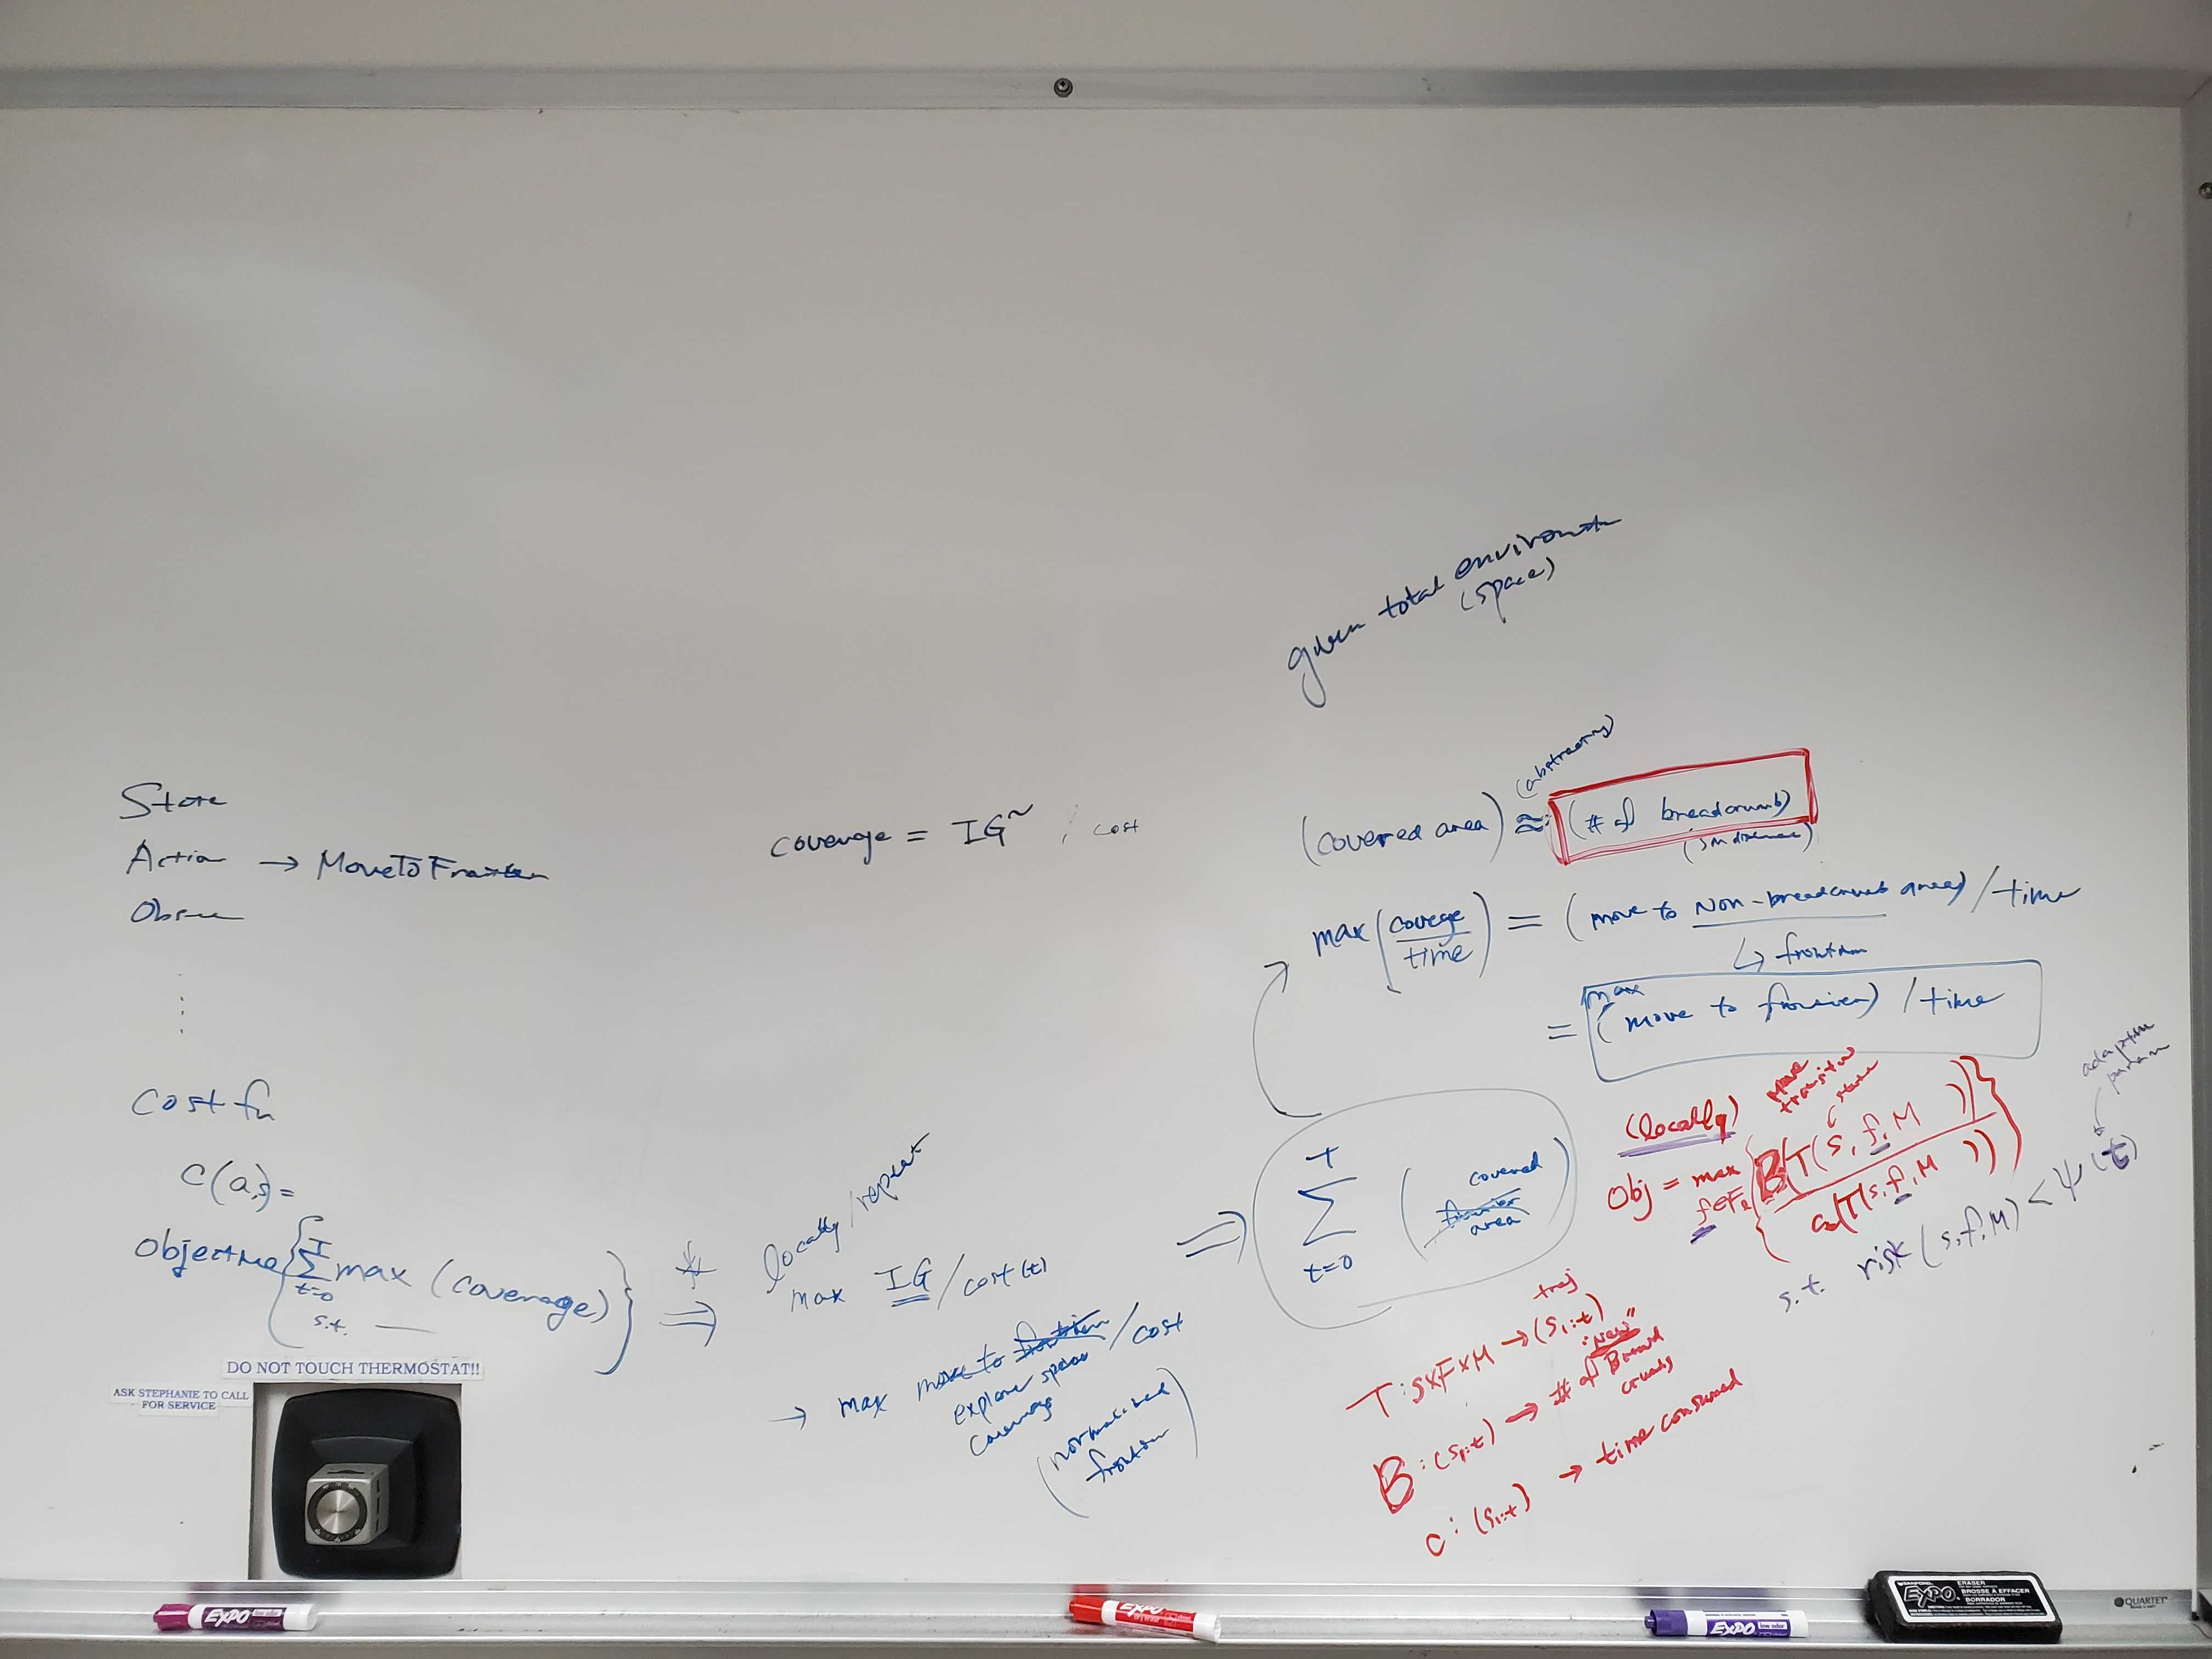
\includegraphics[width=.9\textwidth]{figures/whiteboardA.jpg}
  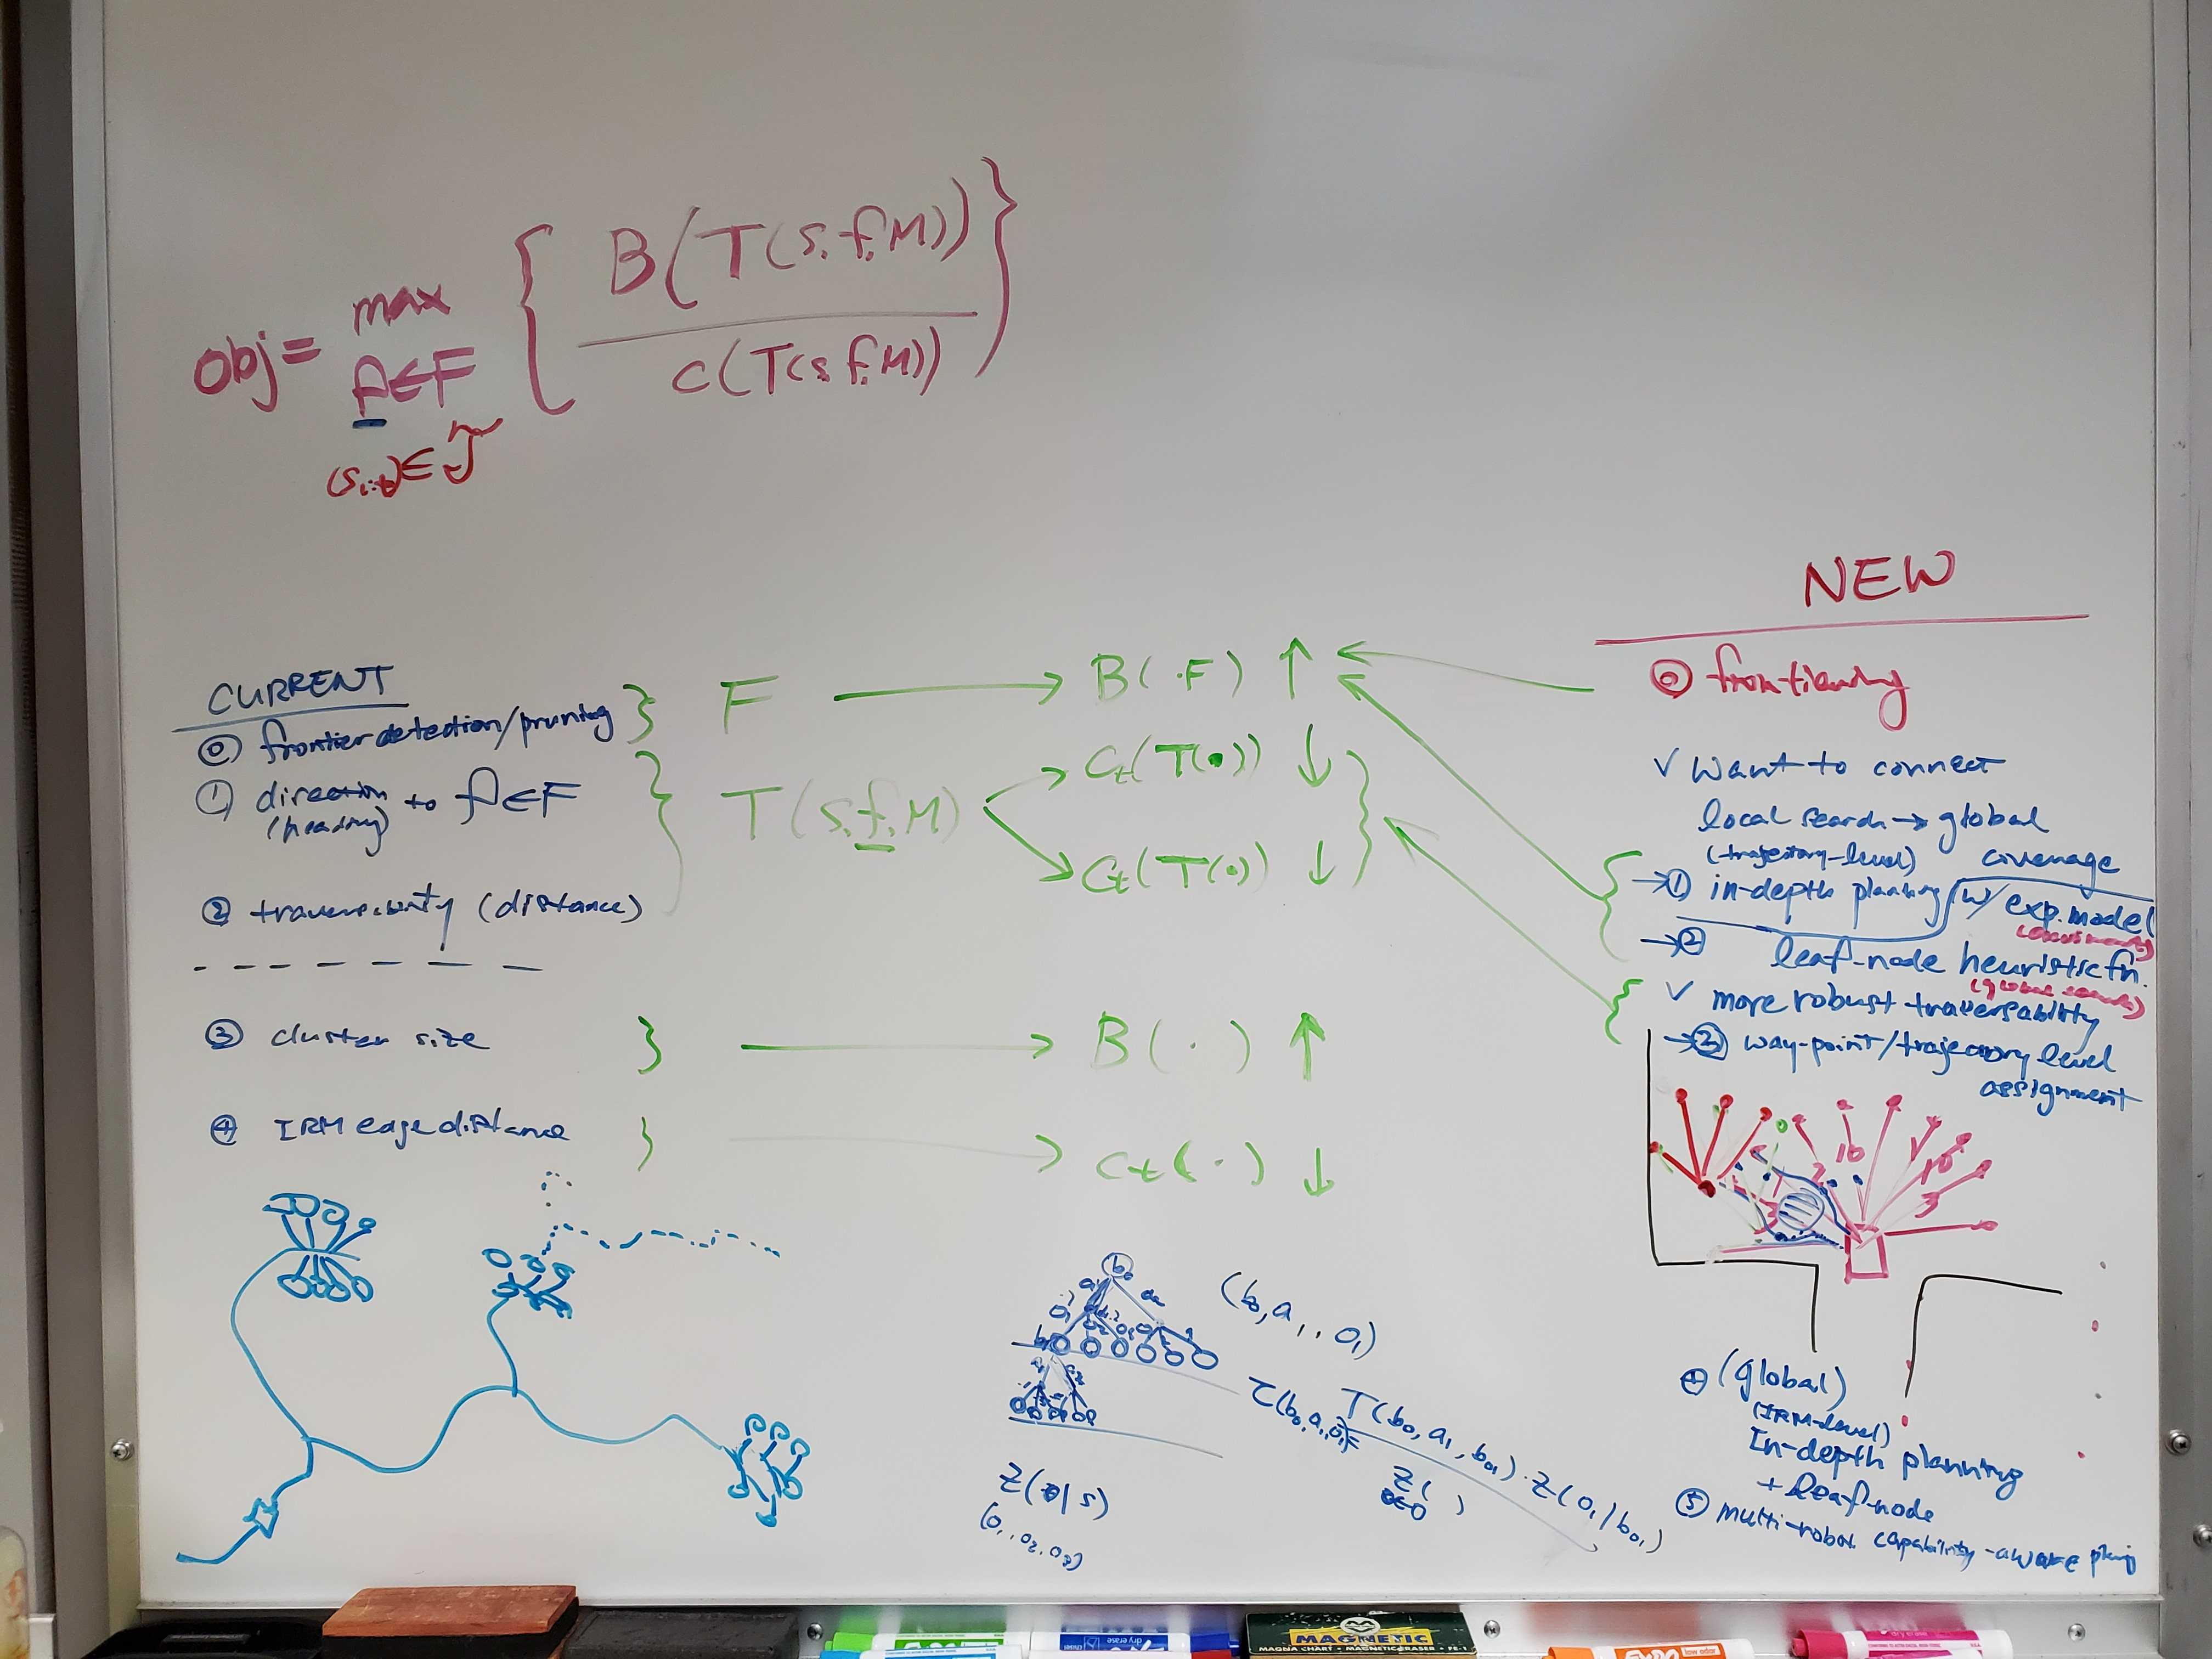
\includegraphics[width=.9\textwidth]{figures/whiteboardB.jpg}
\end{figure}
\clearpage

\clearpage
\begin{figure}[H]
  \centering
  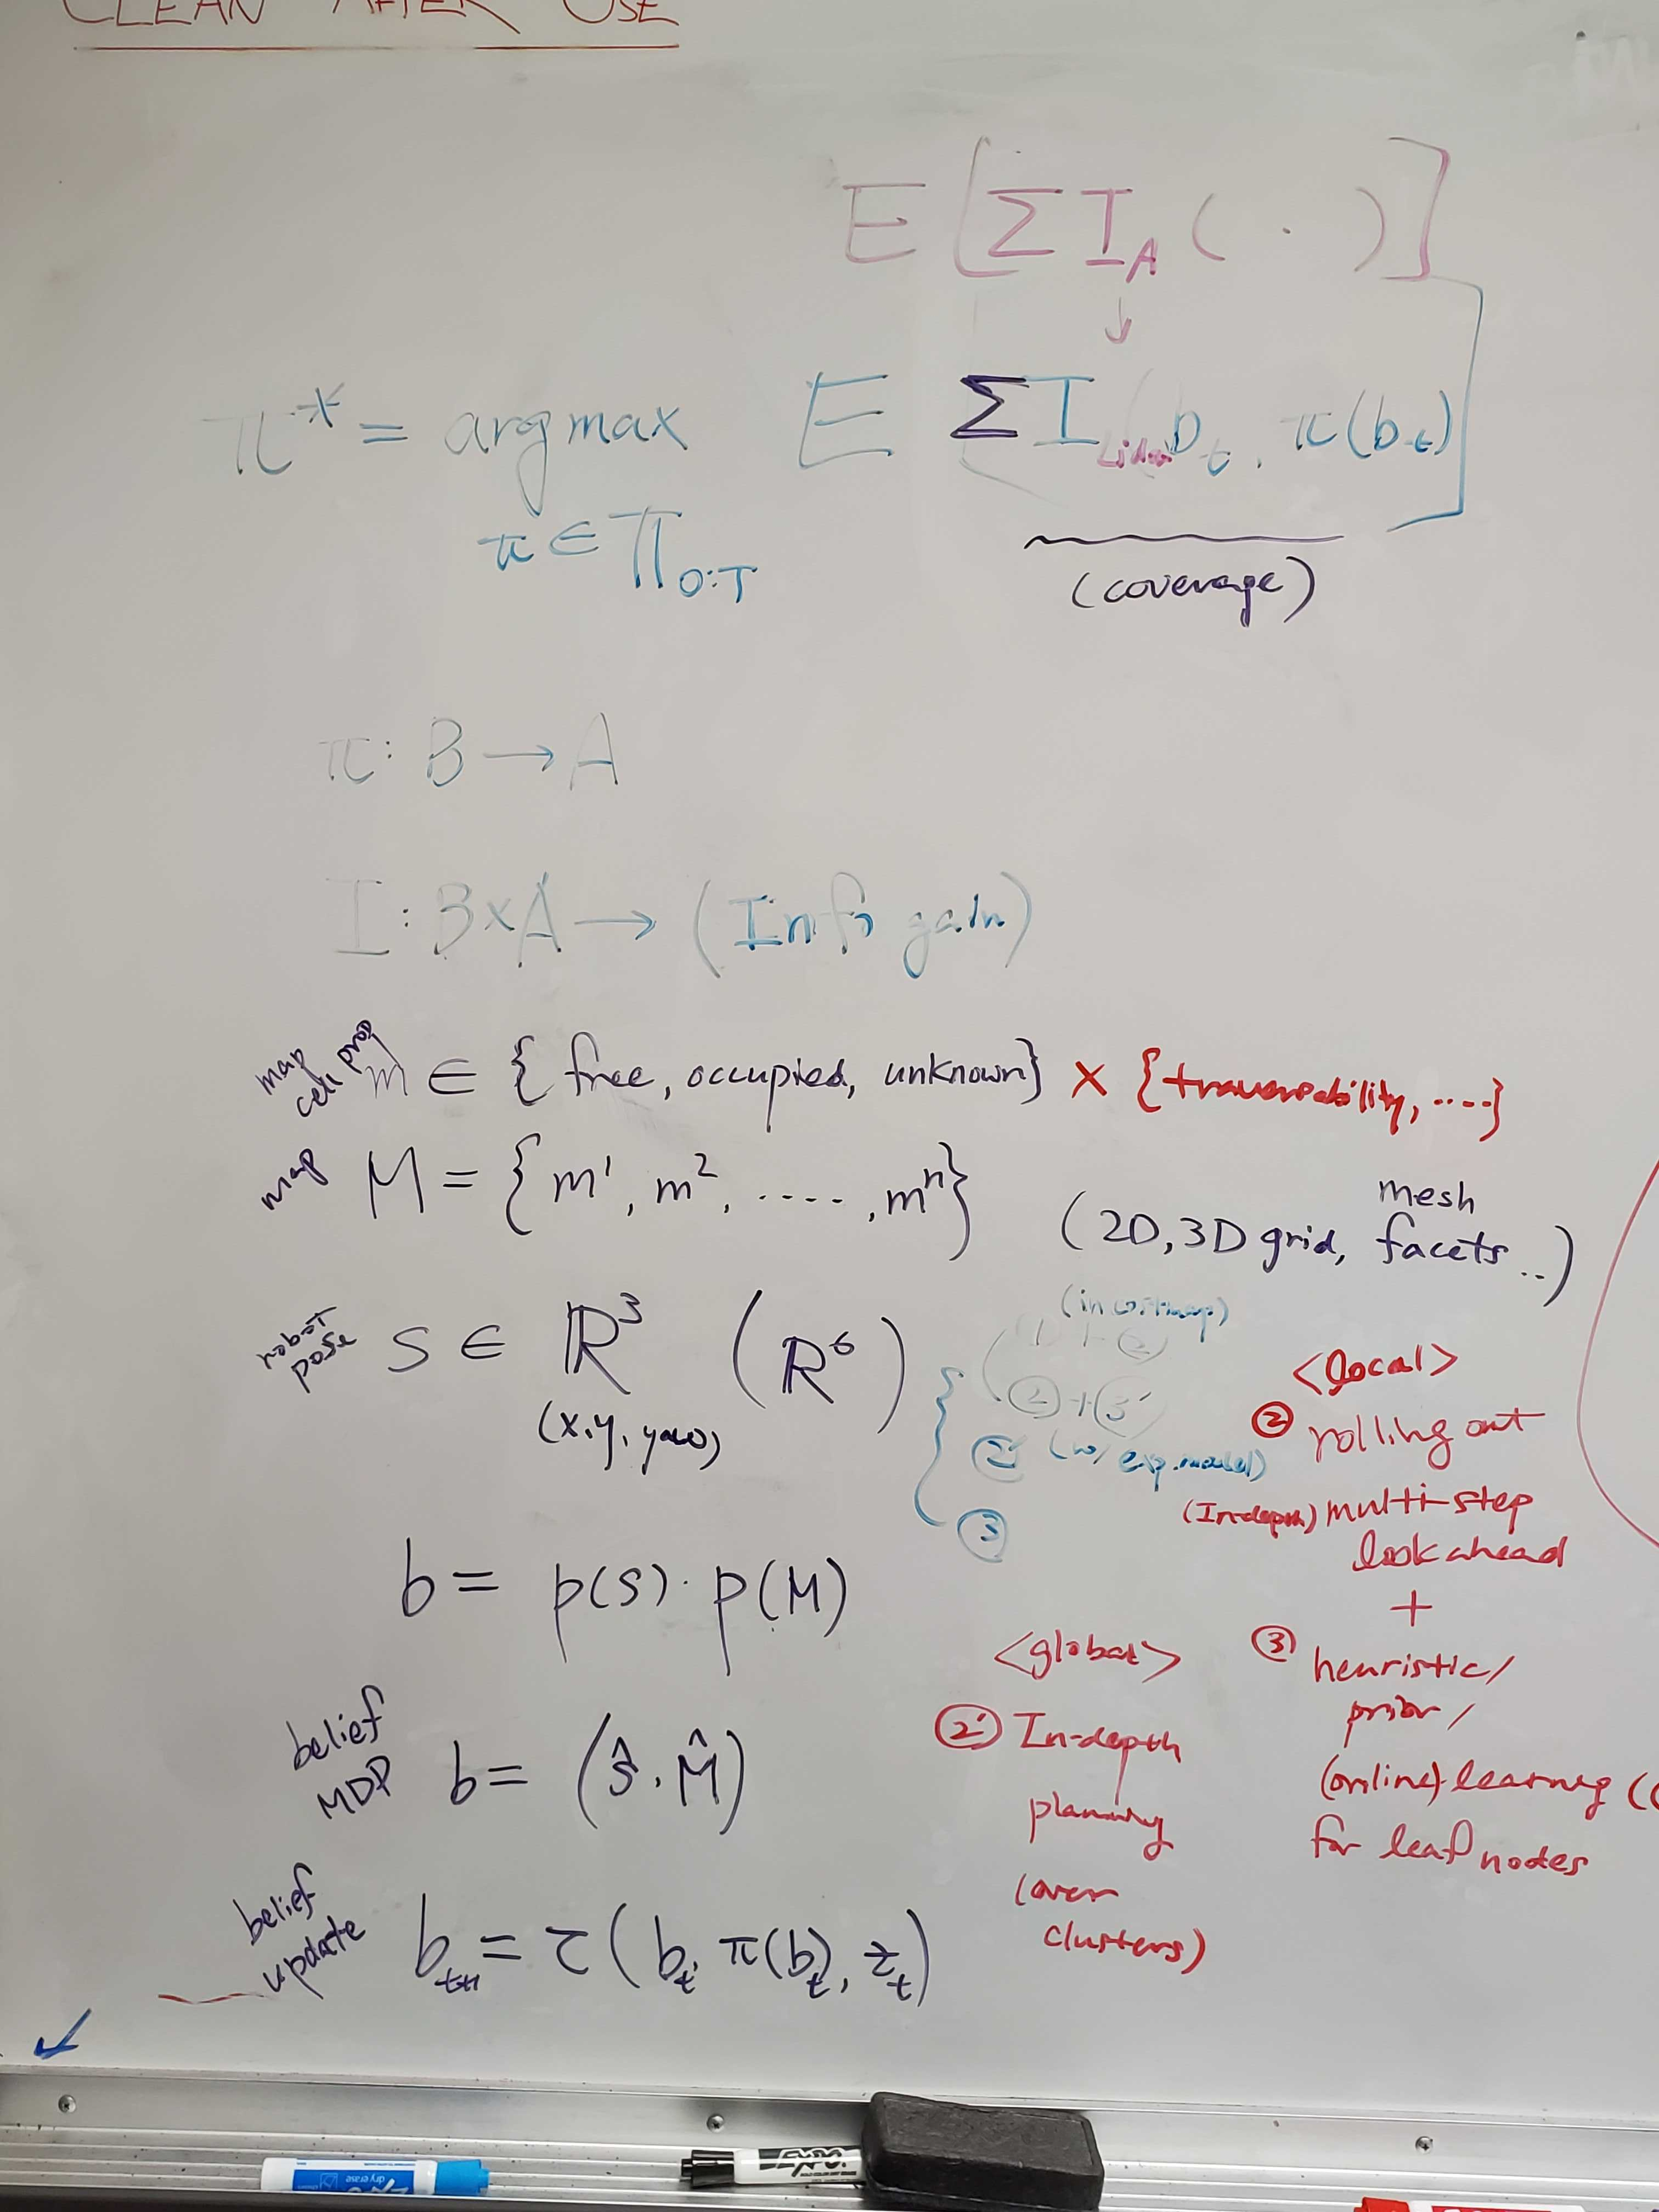
\includegraphics[width=.9\textwidth]{figures/whiteboardI.jpg}
\end{figure}
\clearpage
\begin{figure}[H]
  \centering
  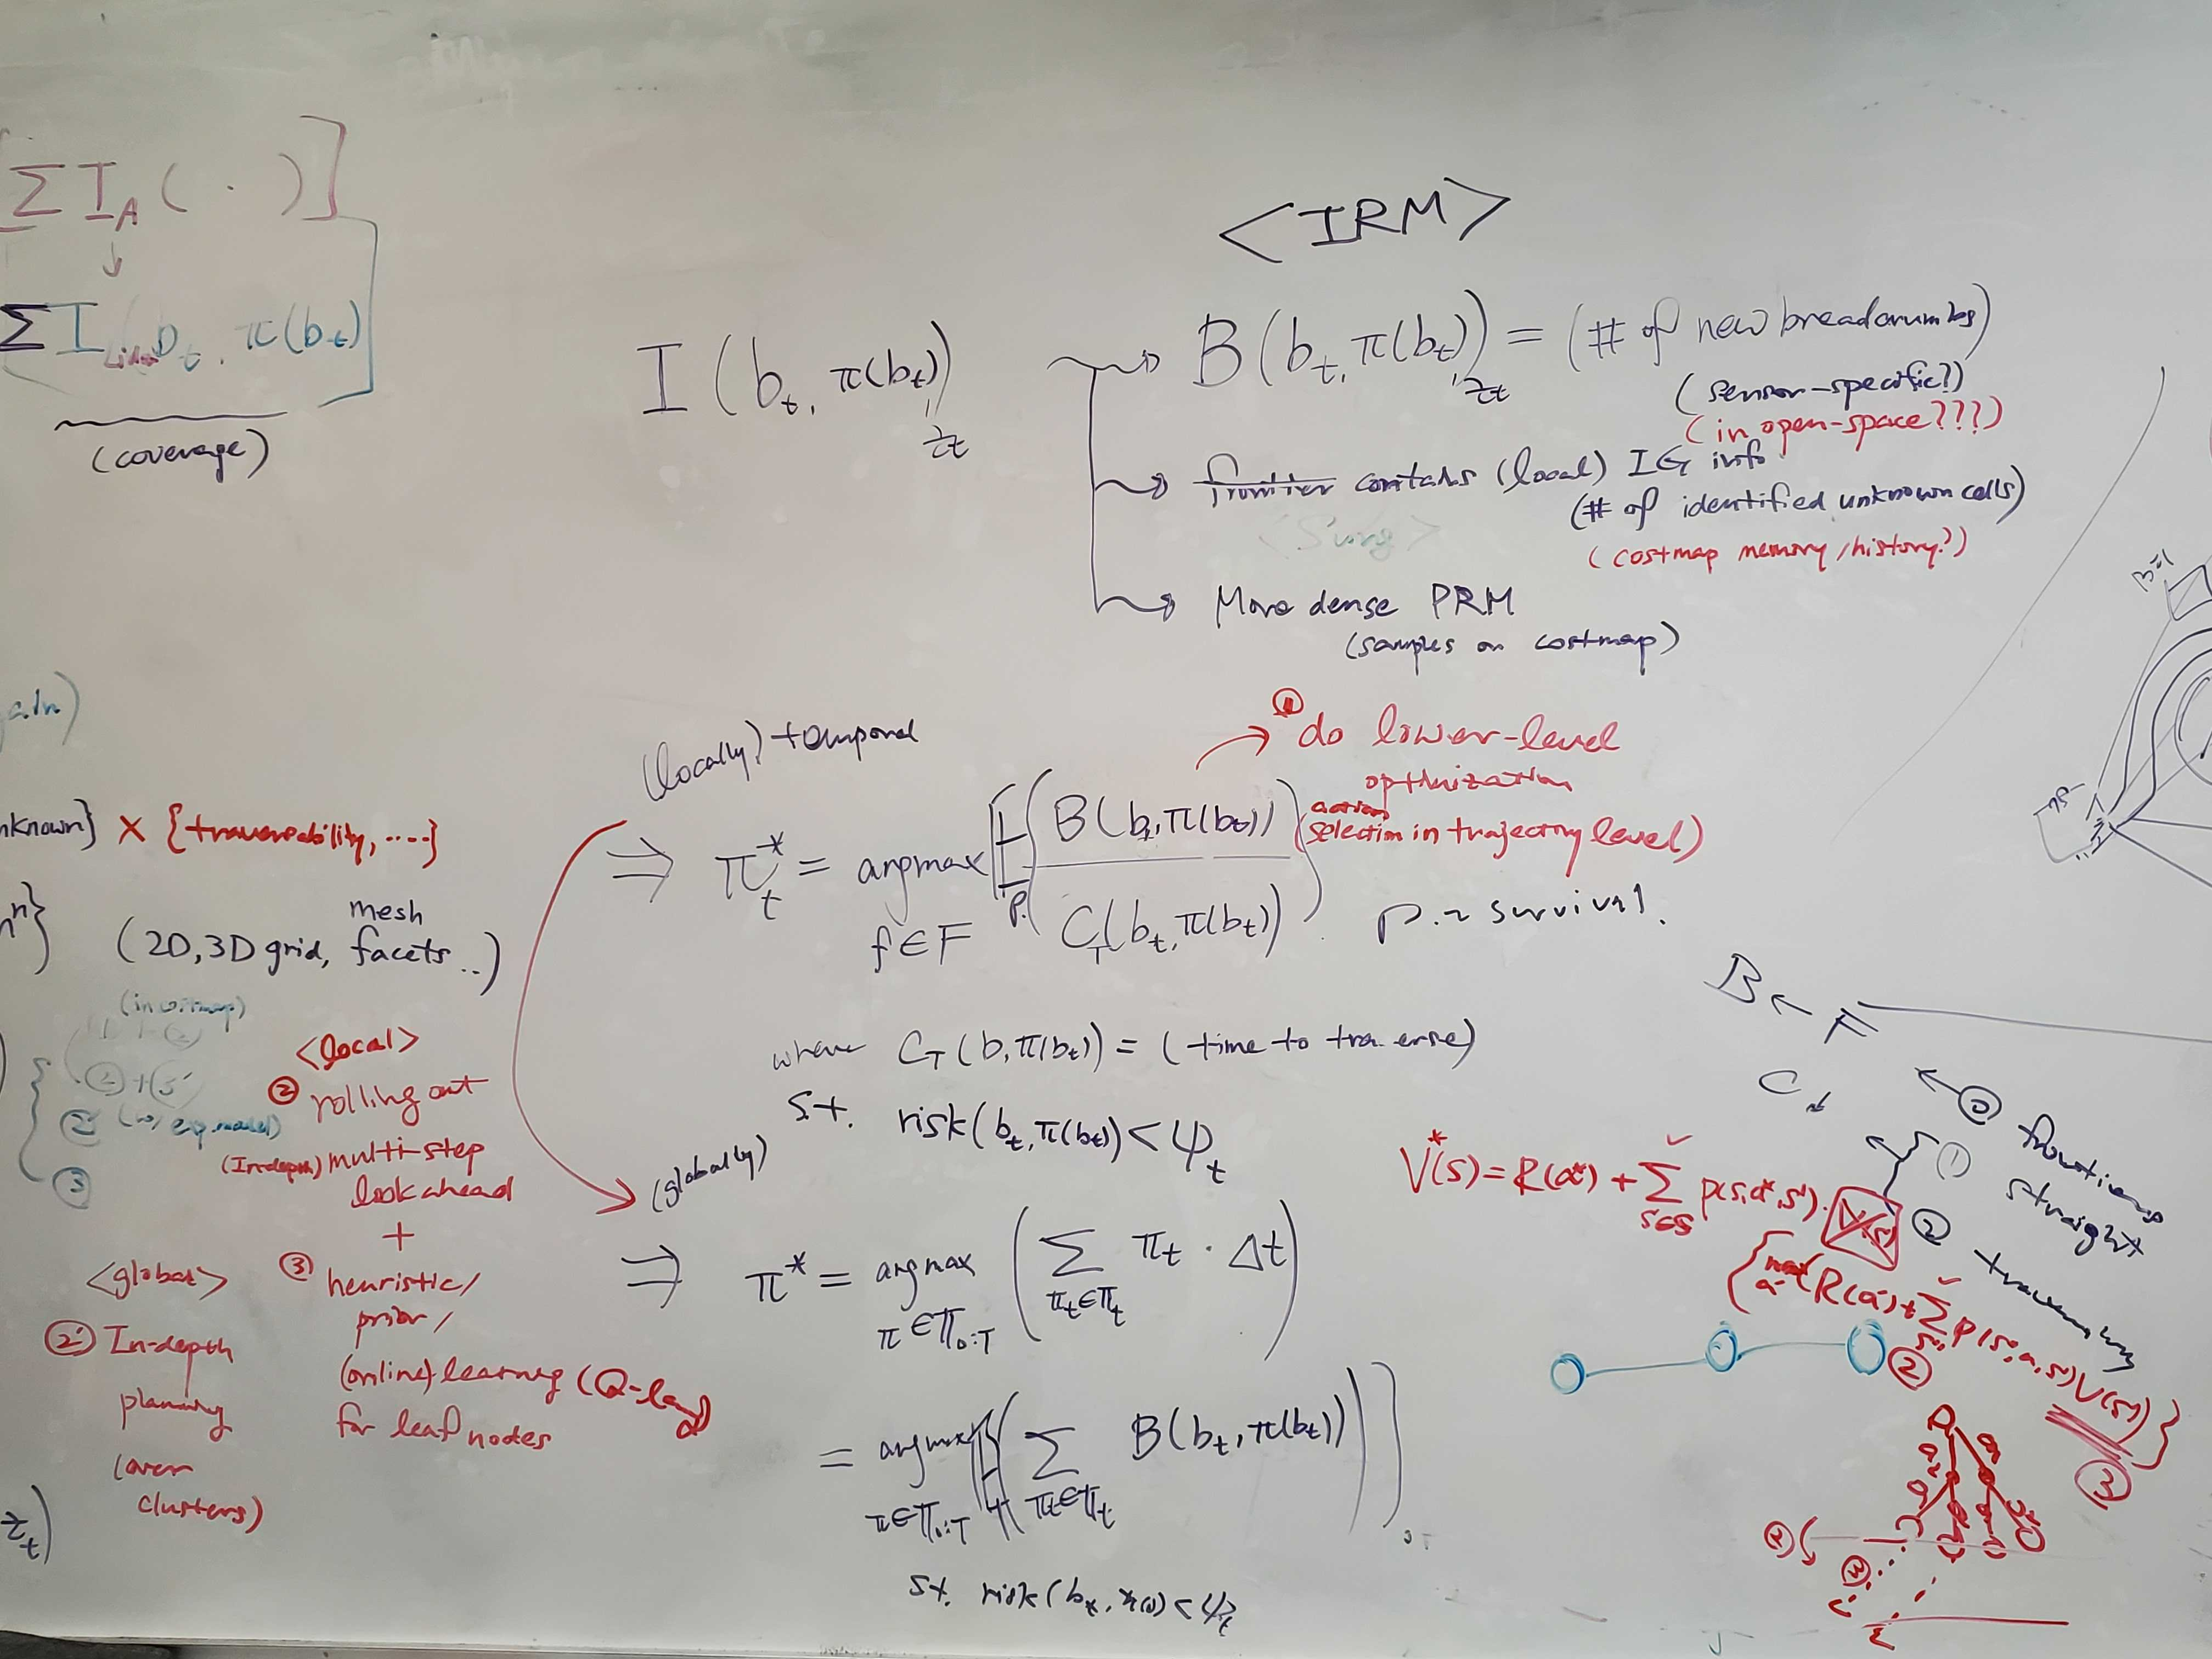
\includegraphics[width=.9\textwidth]{figures/whiteboardII.jpg}
  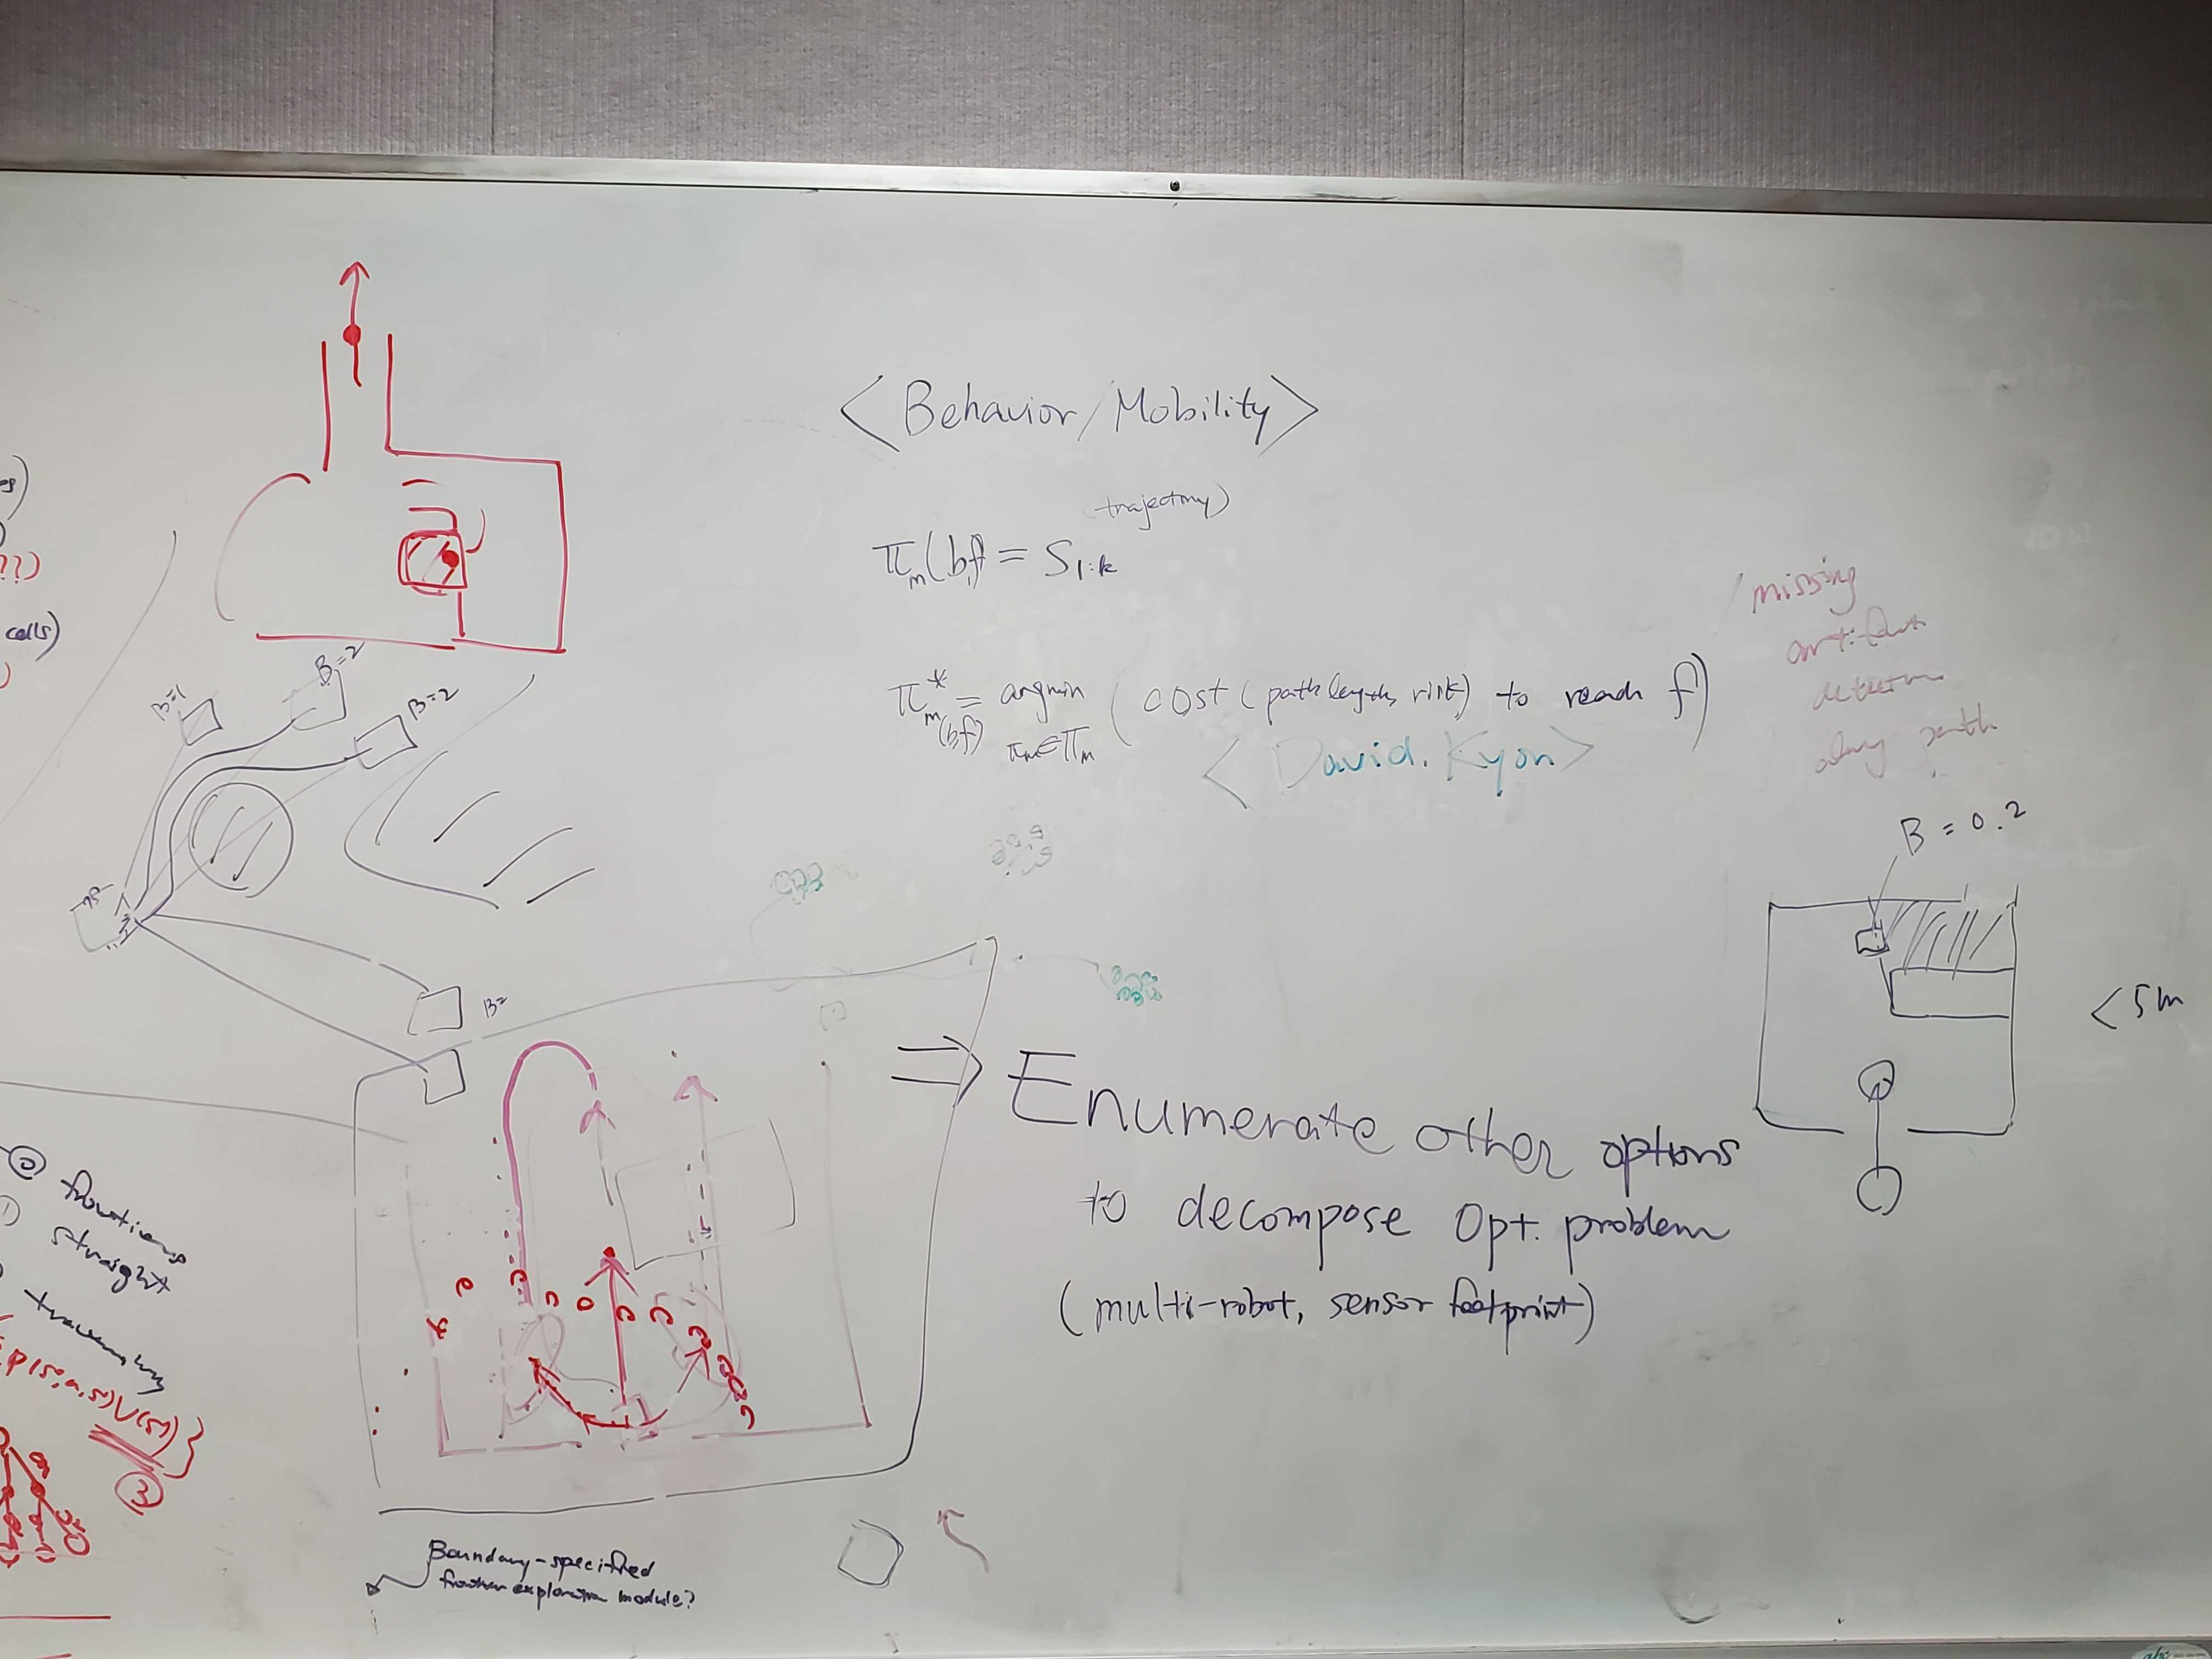
\includegraphics[width=.9\textwidth]{figures/whiteboardIII.jpg}
\end{figure}
\clearpage



% %%%%%%%%%%%%%%%%%%%%%%%%%%%%%%%%%%%%%%%%%%%%%%%%
% \section{High-level instructions}
%
% \begin{verbatim}
%
% 1. What is the problem?
% 2. Why is it relevant?
% 3. Why is it hard?
% 4. What have others done?
% 5. What is missing?
% 6. What is our ONE key insight?
% 7. How do we compare against the state of the art?
% 8. What are our contributions?
% 9. What are our limitations?  
%
% @ Contribution
% - frontier-based autonomous exploration in large-scale unknown environments
%   : sparse-yet-informative graph representation of space for large-scale exploration
%     . resilient to localization error, loop closure, etc.
%     . abstract representation for less memory usage and easier data transfer
%   : frontier-based exploration in the real world
%     . frontier detection/filtering/pruning in complex 3D environment
%     . frontier-based coverage planner, aware of robot's traversability
%
% @ Structure
% - introduction
% - frontiering
%   : IRM - graphical space representation
%   : frontier segment detection
%   : frontier node sampling/filtering/pruning
% - coverage planner
%   : problem formulation
%   : local search
%   : global search
% - experimental results
% - conclusion
%
% \end{verbatim}
% \clearpage{}


\bibliographystyle{unsrt}
\bibliography{references}




\end{document}
